\documentclass[11pt]{amsart}

\usepackage[T1]{fontenc}
\usepackage{amsmath,amssymb,amsthm}
\usepackage{graphicx}
\usepackage{float}
\usepackage{booktabs}
\usepackage[dvipsnames]{xcolor}
\usepackage[colorlinks=true,linkcolor=blue,citecolor=blue,urlcolor=blue]{hyperref}

\usepackage[left=2.1cm,right=2.1cm,top=2.9cm,bottom=2.9cm]{geometry}

% ---------------------------------------------------------------------------
% Changes made for Reviewer #1 (round 2) are typeset in blue.
\newcommand{\rev}[1]{\textcolor{blue}{#1}}
\newenvironment{revblock}{\color{blue}}{}
% ---------------------------------------------------------------------------

\theoremstyle{definition}
\newtheorem{definition}{Definition}
\theoremstyle{remark}
\newtheorem{remark}{Remark}
\theoremstyle{plain}
\newtheorem{theorem}{Theorem}
\newtheorem{proposition}[theorem]{Proposition}
\newtheorem{corollary}[theorem]{Corollary}
\newtheorem{lemma}[theorem]{Lemma}

\newcommand{\R}{\mathbb{R}}
\newcommand{\N}{\mathbb{N}}
\DeclareMathOperator{\dist}{dist}

\begin{document}

\title{A PINNs approach for the computation of eigenvalues in elliptic problems}

\author{Juli\'an Fern\'andez Bonder}
\address{Departamento de Matem\'atica, Facultad de Ciencias Exactas y Naturales, Universidad de Buenos Aires, Buenos Aires, Argentina, and Instituto de C\'alculo UBA-CONICET, Buenos Aires, Argentina}
\email{jfbonder@dm.uba.ar}

\author{Ariel Salort}
\address{Departamento de Matem\'aticas Aplicadas y Ciencia de Datos, Universidad San Pablo-CEU, CEU Universities, Juli\'an Romea 2, 28003 Madrid, Spain}
\email{ariel.salort@ceu.es}

\subjclass[2020]{35P05, 35P30, 35J92, 65N25, 68T07}
\keywords{Physics-informed neural networks; eigenvalue problems; elliptic PDEs; $p$-Laplacian; deep learning}

\begin{abstract}
\begin{revblock}
We propose a method for computing eigenvalues of elliptic operators with physics-informed neural
networks (PINNs). For a fixed value $E$ of the spectral parameter, the squared residual of the
equation is minimized over network functions that satisfy the Dirichlet condition exactly; the
resulting loss curve $\Lambda(E)$ equals $\dist(E,\sigma)^2$ for self-adjoint operators, so the
eigenvalues are its zeros and any spectral window can be targeted without computing the lower
eigenvalues. We analyse the penalized loss used in practice: its loss curve is given in closed form,
which shows that the variational problem has no spurious local minima and yields a rule for the
penalty parameter ($\mu\ge D^2$, where $D$ is the largest distance from the scanned window to the
spectrum, with collapse of the network for $\mu<D^2/2$); we prove a stability result for the
detection under training and sampling errors, and use the Weinstein and Kato--Temple inequalities as
a posteriori certificates for each detected eigenvalue. Experiments in dimensions two to four (disk,
square, triangle, annulus, balls, harmonic and well potentials) give relative errors between
$10^{-6}$ and $5\cdot10^{-3}$ with respect to exact values, and agree to within $0.1\%$ with
independent finite element computations for the double-well, four-well and harmonic potentials.
For the $p$-Laplacian, $p=2.2$ and $p=2.5$, the method reproduces the known first and second
eigenvalues to within $0.1\%$ and detects further eigenvalues (third to fifth minima in the disk),
each matched by an independent reference; we identify the dominant error sources (optimization noise
and a residual floor at the critical points of the network) and show that the method works for
$p\ge2$ but not for $p=1.5$. A cost comparison shows that a Rayleigh-quotient PINN with deflation is
cheaper for the lowest eigenvalues and resolves multiplicities; the advantages of the scan are its
parallelism, per-eigenvalue certificates, direct access to high eigenvalues, and its applicability
to nonlinear problems.
\end{revblock}
\end{abstract}

\maketitle

\section{Introduction}

The impact of artificial intelligence (AI) on everyday life has become undeniable in recent years. From smartphones to image recognition, from medical diagnostics to self-driving cars, machine learning, and deep learning in particular, has transformed the way we interact with technology.

This influence has also extended into mathematics and physics, where machine learning techniques are being applied to analyze complex phenomena that were traditionally approached using classical analytical methods. Among these, problems governed by partial differential equations (PDEs) are especially prominent, due to their central role in modeling physical systems across many disciplines. Reflecting this trend, a growing number of software libraries and frameworks have been developed as educational and research tools for solving PDE-based problems in computational science and engineering; see, for instance, \cite{Lu-Meng-Mao, Rackauckas, Rackauckas-Innes-Ma-Bettencourt-etal} and references therein.

In parallel, neural network-based approaches for approximating solutions to PDEs have gained
increasing attention. These include successful applications to problems such as the Burgers,
Eikonal, and heat equations \cite{Blechschmidt-Ernst}, linear diffusion equations in complex
two-dimensional geometries \cite{Berg-Nystrom}, and nonlinear problems such as three-dimensional
PDEs, Emden--Fowler systems, and fractional-order predator--prey models \cite{GT24, KKG, MHO}.
\rev{Nonlinear dispersive models, such as the generalized higher-order nonlinear Schr\"odinger
equation, whose multi-peak and breather-type solitary waves were recently studied in
\cite{Yasin-etal}, are further natural targets for such solvers.}

A natural extension of this idea is the use of neural networks (NNs) as general-purpose function approximators for solving differential equations. A prototypical example arises in quantum mechanics, where one seeks to solve the eigenvalue problem
\begin{equation}\label{eigen}
-\Delta u + V(x) u = E u,\quad \text{in } \R^{\rev{d}},
\end{equation}
with a given potential function \( V \colon \R^{\rev{d}} \to \R \) and eigenvalue parameter \( E \in \R \). The idea of employing NNs to approximate solutions of such equations dates back to the 1990s \cite{Lagaris-Likas-Fotiadis}, but the field gained significant momentum with the introduction of {\em Physics-Informed Neural Networks} (PINNs) in \cite{Raissi-Perdiakaris-Karniadakis}, which triggered a wave of research and applications (see also \cite{Karniadakis-etal}).
\rev{In all the examples below the problem is posed in a bounded domain $\Omega$ with homogeneous
Dirichlet boundary conditions, also when a potential $V$ is present.}

Most early PINN-based work focused on source problems, where the term \( E u \) in \eqref{eigen} is replaced by a known forcing function \( f \). The eigenvalue problem itself has been more recently addressed: first in one dimension \cite{Jin-Mattheakis-Protopapas1, Jin-Mattheakis-Protopapas2, Sakar}, and later in two dimensions \cite{Holliday-Lindner-Ditto}. Related approaches have also been proposed in \cite{Rowan-Evans-Maute-Dootsan}, which include extensions to nonlinear eigenvalue problems\rev{; the Deep Ritz method \cite{E-Yu} also treats eigenvalue problems through the Rayleigh quotient}.

Several methodologies have been proposed to address eigenvalue problems using neural networks.
The approach in \cite{Sakar} constructs a trial wavefunction that automatically satisfies the boundary conditions, represents the unknown component with a neural network, and trains the network by minimizing an appropriately defined loss function.
%
In \cite{Jin-Mattheakis-Protopapas1, Jin-Mattheakis-Protopapas2}, the authors introduce an unsupervised neural network architecture that simultaneously learns both the eigenvalues and the corresponding eigenfunctions through a scanning mechanism.
%
Alternatively, \cite{Rowan-Evans-Maute-Dootsan} employs a neural network to discretize the eigenfunction and minimize the associated Rayleigh quotient.

\begin{figure}[htbp]
\centering
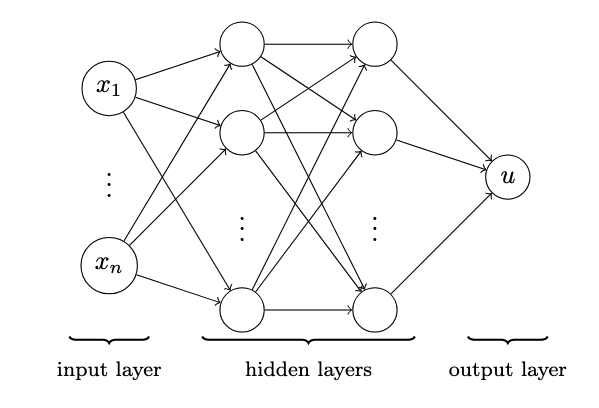
\includegraphics[width=.6\columnwidth]{NN-Tikz.png}
\caption{A fully connected feedforward NN with a \rev{$d$}-dimensional input and a 1-dimensional output.}
\label{NN.fig}
\end{figure}

In these works, the solution \( u \) is approximated using a fully connected feedforward neural network (see Fig.~\ref{NN.fig}), with variations in the number of hidden layers and activation functions across implementations. To approximate the eigenvalue \( E \), the authors minimize the {\em Rayleigh quotient}:
\[
\rev{R}(u) = \frac{\int_{\rev{\Omega}} |\nabla u|^2 + V(x) u^2\, dx}{\int_{\rev{\Omega}} u^2\, dx}.
\]
Minimizing \( \rev{R}(u) \) yields an approximation of the principal eigenvalue \( E_1 \) and its associated eigenfunction \( u_1 \). Higher-order eigenpairs can be computed by iteratively minimizing the same functional while constraining the search to subspaces orthogonal to previously computed eigenfunctions.

This approach, while effective, presents two main limitations:
\begin{enumerate}
\item It is inherently sequential: to compute eigenvalues within a given range, one must first compute all lower ones, which can be inefficient.
\item Its extension to nonlinear problems (such as those involving the \(p\)-Laplace operator) is limited, since orthogonality conditions between eigenfunctions are no longer available.
\end{enumerate}

\begin{revblock}
\noindent\emph{Contributions.} (i) We propose to compute eigenvalues as the zeros of the loss curve
$E\mapsto\inf_u\Lambda(u,E)$, where $\Lambda$ is the squared PDE residual; for self-adjoint
problems $\Lambda(E)=\dist(E,\sigma)^2$ (Section~\ref{sec.approach}). (ii) We compute the loss curve
of the penalized loss used in practice in closed form, show that it has no spurious local minima,
derive a rule for the penalty parameter $\mu$ and verify it in a sensitivity study
(Proposition~\ref{prop.penalized}, Section~\ref{sec.mu}). (iii) We prove a stability result for the
detection of eigenvalues under training and sampling errors, and attach to each computed eigenvalue
an a posteriori enclosure (Weinstein and Kato--Temple; Sections~\ref{sec.certificate} and
\ref{sec.stability}). (iv) We validate the method against exact values and independent finite
element computations in dimensions $2$--$4$ (Section~\ref{sec.examples}), quantify its cost and
compare it with a Rayleigh-quotient PINN with deflation (Section~\ref{sec.cost}). (v) For the
$p$-Laplacian we prove that the zeros of the loss curve are exactly the eigenvalues, compute
eigenvalues beyond the second one and analyse the sources of error (Section~\ref{sec.nolin}).

\noindent\emph{Organization of the paper.} Section~\ref{sec.approach} introduces the loss curve and
the penalized loss. Section~\ref{sec.implementation} describes the implementation, the refinement
of the computed eigenvalue and the a posteriori certificate. Section~\ref{sec.examples} contains
the linear examples (higher eigenvalues, higher dimensions, other geometries and potentials, with
finite element validation). Section~\ref{sec.nolin} treats the $p$-Laplacian. Section~\ref{sec.analysis}
analyses the practical method: stability and spurious minima, choice of $\mu$, and computational
cost. Section~\ref{sec.conclusions} summarizes the results and the limitations. The appendices
contain the existence of minimizers and the proofs of the new propositions.
\end{revblock}


\section{Our approach}\label{sec.approach}

To overcome the drawbacks mentioned above, we propose a different approach to problem \eqref{eigen}. We define the following loss function:
\begin{equation}\label{Lambda}
\Lambda(u, E) = \frac{\int_{\rev{\Omega}} (\Delta u - V(x) u + Eu)^2\, dx}{\int_{\rev{\Omega}} u^2\, dx}.
\end{equation}
Given a fixed $E\in \R$, minimizing with respect to $u$ yields a {\em loss curve}:
\begin{equation}\label{loss-curve}
\Lambda(E) = \inf_u \Lambda(u, E).
\end{equation}
A proof of the existence of a minimizer $u_E$ for \eqref{loss-curve} is provided in Theorem \ref{teo.min} in the appendix.

\begin{revblock}
Let $L=-\Delta+V$, with the Dirichlet condition built into its domain $D(L)$, be self-adjoint with
compact resolvent (this is the case for a bounded domain and bounded $V$), let
$E_1\le E_2\le\cdots$ be its eigenvalues repeated according to multiplicity, $\{u_k\}$ an orthonormal
basis of eigenfunctions, $\sigma=\{E_k\}$ the spectrum and $d(E):=\dist(E,\sigma)$. Writing
$u=\sum_kc_ku_k\in D(L)$,
\[
\Lambda(u,E)=\frac{\sum_k c_k^2 (E_k-E)^2}{\sum_k c_k^2}\ \ge\ \min_k (E_k-E)^2,
\]
with equality if and only if $u$ lies in the eigenspace of the eigenvalue(s) closest to $E$. Hence
\begin{equation} \label{cota.igual}
\Lambda(E)=\min_k (E_k-E)^2=d(E)^2 .
\end{equation}
In particular $\Lambda\ge0$, the zeros of $\Lambda$ are exactly the eigenvalues, every local minimum
of $\Lambda$ is a zero, and $\Lambda$ is a parabola of unit curvature around each eigenvalue. The
curve does not see multiplicities: a multiple eigenvalue produces a single zero.
\end{revblock}

Note that the characterization of eigenvalues as the zeros of $\Lambda$ only uses that
$\Lambda(u,E)$ is the squared residual of the equation, and not the spectral decomposition
above. Hence the same mechanism applies to nonlinear eigenvalue problems, where no
orthogonality between eigenfunctions is available, as shown in \rev{Section~\ref{sec.nolin}}. In the nonlinear case there is no spectral decomposition, so the identity
\eqref{cota.igual} is no longer available. What survives is the mechanism
itself: the loss vanishes exactly at the eigenvalues \rev{(Proposition~\ref{prop.plap})}, so they can still be
detected as the minima of the loss curve.

Having defined $\Lambda(E)$, the eigenvalues can be found just by scanning $E$ and locating the local minima of $\Lambda$,
with no need to know the lower ones. This is the \rev{main strength} of the proposed method.
\rev{The idea of scanning a spectral parameter and locating the minima of a residual is classical
in other contexts (e.g.\ the method of particular solutions \cite{Betcke-Trefethen} and the folded-spectrum method \cite{Wang-Zunger}); here
it is combined with a neural network ansatz, which makes it applicable in several dimensions and to
nonlinear operators.}

In Fig.~\ref{Lambda.fig}, the \rev{curve $\Lambda(E)$} for problem \eqref{eigen} is plotted in the two-dimensional case with \rev{the hard-wall} potential given by $V(x)=0$ for $|x|\le 1$ and $V(x)=\infty$ for $|x|>1$.  In this case the eigenvalues are known explicitly. The first four \rev{distinct eigenvalues} are:
$$
 E_1 = 5.7832,\ E_2 = \rev{14.6820},\ E_3 =  26.3746,\ E_4 =  30.4713
 $$
\rev{($E_2$ and $E_3$ are double).}
\begin{figure}[htbp]
\centering
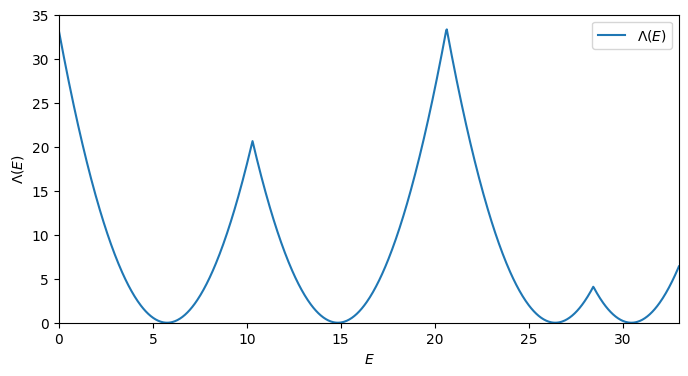
\includegraphics[width=.6\columnwidth]{Loss.png}
\caption{The \rev{exact} loss curve $\Lambda(E)\rev{=\min_k(E-E_k)^2}$ \rev{for the Dirichlet Laplacian in the unit disk}.}
\label{Lambda.fig}
\end{figure}
Our approach proceeds as follows:

We first fix the interval $[E_*, E^*]$  where the eigenvalues are expected to lie. Then, we take a uniform partition of this interval:
$$
E_*=E^1<E^2<\cdots<E^{\rev{J}}=E^*,
$$
and for each $E^i$ we train our neural network to minimize $\Lambda(u, E^i)$, obtaining a corresponding minimizer $u^i$.

\rev{Finally, we look for the local minima of the discrete loss curve $\Lambda(E^i)$ whose value is below a threshold. By \eqref{cota.igual} and Proposition~\ref{prop.stability} below, each of them lies within a computable distance of an eigenvalue; the eigenvalue is then refined from the trained network (Section~\ref{sec.certificate}), and the associated minimizers $u^i$ approximate the corresponding eigenfunctions.}

\rev{The aim of this article is to give an approach to compute eigenvalues based on neural networks
whose implementation is simple and which does not require the previously computed eigenvalues.
Our goal is not to obtain the best estimates for linear problems (for that aim there are efficient
and well-studied methods based on finite differences/elements, see Section~\ref{sec.fem}). However,
the method is flexible and has the following features:}
\begin{enumerate}
\item  Unlike the aforementioned methods, our approach allows the computation of higher eigenvalues without requiring the prior computation of lower ones.

\item \rev{The implementation is the same in every dimension; we report experiments in dimensions two, three and four.}

\item \rev{The same code handles different potentials and geometries; only the boundary factor $B$ changes.}

\item The neural network architecture employed in our implementation is simple and extends naturally to nonlinear cases. \rev{While we do not claim more accuracy than existing methods, this allows us to compute eigenvalues of the $p$-Laplacian beyond the second one (Section~\ref{sec.nolin}).}

\item \rev{Each computed eigenvalue comes with an a posteriori bound in the linear case (Section~\ref{sec.certificate}), and the computations at different values of $E$ are independent and can be run in parallel (Section~\ref{sec.cost}).}

\item \rev{In principle, the approach can be adapted to more general operators beyond the $p$-Laplacian.}
\end{enumerate}
\rev{Its limitations (cost compared with Rayleigh-quotient methods for the lowest eigenvalues,
multiplicities and close clusters not resolved) are discussed in Sections~\ref{sec.analysis} and
\ref{sec.conclusions}.}


\section{Implementation details}\label{sec.implementation}

We consider a fully connected neural network, implemented as a feed-forward multilayer perceptron with three hidden layers. Each hidden layer contains 128 neurons with $\tanh$ activation functions. The network maps a spatial coordinate $x\in \R^d$ to a scalar output and is defined as $
x \mapsto \text{NN}(x) \in \mathbb{R}$. All linear layers are initialized using Xavier uniform initialization with the appropriate gain for the tanh activation, and all biases are set to zero.

To enforce the homogeneous Dirichlet boundary condition on the domain $\Omega$, the raw network output $\text{NN}(x)$ is multiplied by a boundary factor $B(x)$, chosen so that
$$
B(x)=0 \text{ for all } x\in\partial\Omega, \qquad B(x)>0 \text{ for all } x\in\Omega.
$$
This construction ensures that the final approximation automatically vanishes on the boundary. Thus, the network returns
$$
u(x)=B(x)\,\text{NN}(x).
$$
\begin{revblock}
The factors used for the domains of this paper are smooth functions vanishing exactly on
$\partial\Omega$ and comparable to the distance to the boundary:
\[
\begin{array}{ll}
\text{Domain} & B(x)\\ \hline
\text{Ball } \{|x|<1\}\subset\R^d,\ d=2,3,4 & 1-|x|^2\\
\text{Square } (0,a)^2,\ a=1,2 & x_1(a-x_1)\,x_2(a-x_2)\\
\text{Triangle with vertices } (0,0),(1,0),(0,1) & x_1x_2(1-x_1-x_2)\\
\text{Annulus } \{r_0<|x|<r_1\} & (|x|-r_0)(r_1-|x|)
\end{array}
\]
Since $u=B\,\mathrm{NN}$ satisfies the boundary condition exactly and is smooth, every network
function belongs to the domain $D(L)$ of the operator; this is what makes the a posteriori bounds of
Section~\ref{sec.certificate} applicable to the trained networks.
\end{revblock}

We begin by studying the \rev{simplest} case, \rev{the hard-wall potential}
\begin{equation}\label{conf.V}
V(x) = \begin{cases}
0 & \text{if } x\in \Omega\\
\infty & \text{if } x\not\in \Omega,
\end{cases}
\end{equation}
which is equivalent to solving the Helmholtz problem with homogeneous Dirichlet boundary condition:
\begin{equation}\label{eigen2}
\begin{cases}
-\Delta u = E u & \text{in }\Omega\\
u=0 & \text{on }\partial\Omega.
\end{cases}
\end{equation}

To ensure normalization, we include a penalization term in the loss function to enforce $\|u\|_2=1$. The resulting loss is:
\begin{equation}\label{lossmu}
\bar \Lambda(u, E) = \int_\Omega (\Delta u \rev{-Vu} + Eu)^2\, dx + \mu\left(\int_\Omega u^2\, dx - 1\right)^2.
\end{equation}
All integrals are approximated using a Monte Carlo scheme, typically using 5000 sampling points.
\rev{(In the code the integrals are replaced by sample means, i.e.\ by integrals with respect to
$dx/|\Omega|$; all statements below are invariant under this change of measure.) For the unit disk
we used $\mu=100$; the choice of $\mu$ is analysed in Section~\ref{sec.mu}.}

\begin{revblock}
\begin{proposition}[Loss curve of the penalized loss]\label{prop.penalized}
Let $\mu>0$, $E\in\R$ and $d=d(E)$. Then
\[
\bar\Lambda(E):=\inf_{u\in D(L)}\bar\Lambda(u,E)=
\begin{cases}
d^2-\dfrac{d^4}{4\mu} & \text{if } d^2\le 2\mu,\\[2mm]
\mu & \text{if } d^2\ge 2\mu .
\end{cases}
\]
If $d^2<2\mu$ the minimizers are the functions $u$ in the eigenspace(s) of the eigenvalue(s)
closest to $E$ with $\|u\|_2^2=1-d^2/(2\mu)$; for them $\Lambda(u,E)=d^2$ and the residual term
equals $d^2(1-d^2/(2\mu))$. If $d^2\ge2\mu$ the unique minimizer is $u=0$. Moreover, for every $E$
all local minimizers of $\bar\Lambda(\cdot,E)$ in $D(L)$ are global minimizers, and every other
critical point is a saddle point.
\end{proposition}
The proof is given in Appendix~\ref{app.proofs}. Thus, at the level of the continuous problem the
landscape has no spurious local minima, the zeros of $\bar\Lambda$ are exactly the eigenvalues for
every $\mu>0$, and the only artifact introduced by the penalty is the trivial state $u=0$, which is
the minimizer when $d(E)^2\ge2\mu$. Spurious minima observed in practice can therefore only come
from the network parametrization, the optimizer or the sampling (Section~\ref{sec.stability}).
\end{revblock}

As described in the previous section, we train the NN to minimize $\bar\Lambda(u, E)$ for each value in a discrete partition $E_* = E^1<\cdots<E^{\rev{J}}=E^*$. To improve efficiency, for each $E^i$, the network is initialized with the weights and biases obtained from training at $E^{i-1}$ \rev{(warm start); in some scans the network is re-initialized every 15--60 grid points}.

The model parameters are optimized using the Adam optimizer \rev{with constant learning rate $10^{-3}$} over a maximum of 3,000 epochs \rev{(one epoch is one Adam step; 2000--5000 epochs depending on the example)}. During each epoch, 5,000 spatial points are dynamically sampled to compute the loss, residual, and norm. An early stopping mechanism terminates training if the loss fails to improve by at least \rev{$\mathrm{tol}=10^{-5}$} across 300 consecutive epochs; \rev{these settings are used in all the linear examples unless stated otherwise.} Upon completion of training, we obtain the discrete loss curve
$$
\bar \Lambda(E^i)=\bar\Lambda(u^i, E^i)\rev{,}
$$
and each local minimum below a given threshold $\epsilon>0$ is taken as an approximate eigenvalue for \eqref{eigen2}.
\rev{The threshold was chosen per example after inspecting the curve; Proposition~\ref{prop.stability}
shows what any choice guarantees, and the certificate of Section~\ref{sec.certificate} makes the
threshold unnecessary for accepting a detection. In the tables we report, besides the computed
eigenvalue, the value $\mathrm{Residual}=\frac1N\sum_{i=1}^N(\Delta u-Vu+Eu)^2(x_i)$ of the first
term of \eqref{lossmu}; since $\frac1N\sum u(x_i)^2\approx1$ at the minima,
$\mathrm{Residual}\approx\Lambda(u,E)=r^2$, where $r$ is the residual norm defined in
Section~\ref{sec.certificate}.}
\begin{figure}[htbp]
\centering
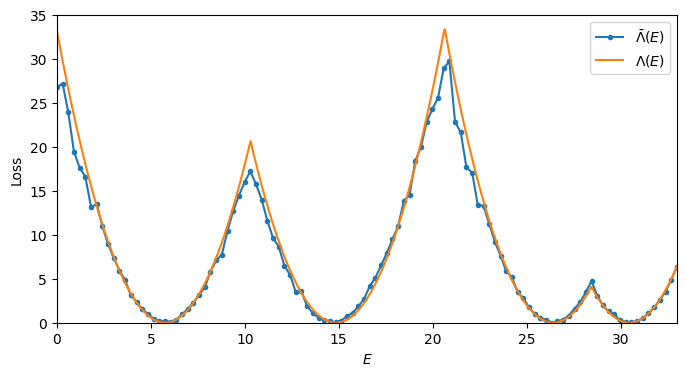
\includegraphics[width=.7\columnwidth]{lossNN-lento.png}
\caption{The loss curve $\bar\Lambda(E)$ \rev{in the unit disk (Dirichlet Laplacian)} compared with the \rev{exact curve $\Lambda(E)=\min_k(E-E_k)^2$; near the peaks the penalized curve lies below $\Lambda(E)$, as predicted by Proposition~\ref{prop.penalized}}.}
\label{lossNN.fig}
\end{figure}

Fig.~\ref{lossNN.fig} shows the loss curve $\bar\Lambda(E^i)$ in the case where $\Omega$ is the unit disk in $\R^2$. \rev{The grid locates the eigenvalues up to its resolution; the value is then refined as described in Section~\ref{sec.certificate}.}
The associated computed eigenfunctions are displayed in Fig.~\ref{func.fig}\rev{.}

\begin{figure}[htbp]
\centering
\begin{tabular}{cccc}
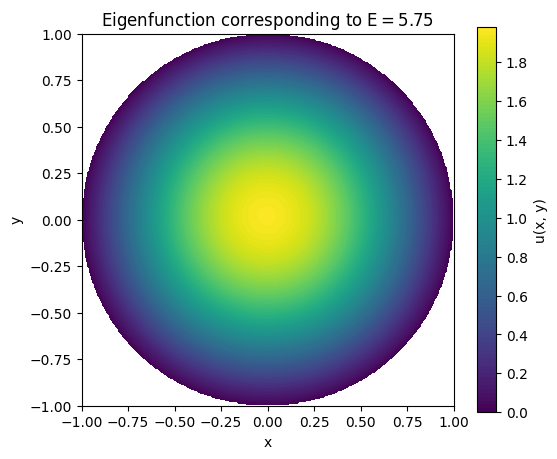
\includegraphics[width=.2\columnwidth]{eigen1-1.png} & 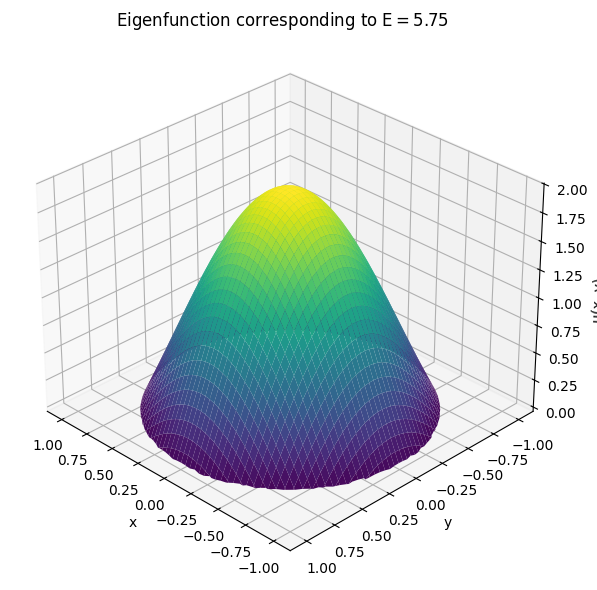
\includegraphics[width=.2\columnwidth]{eigen1-2.png} &
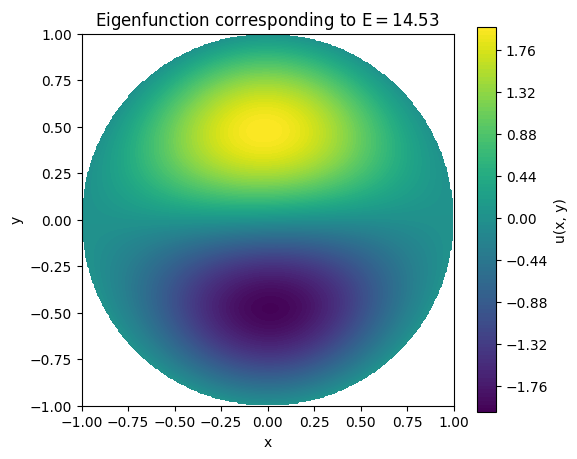
\includegraphics[width=.2\columnwidth]{eigen2-1.png} & 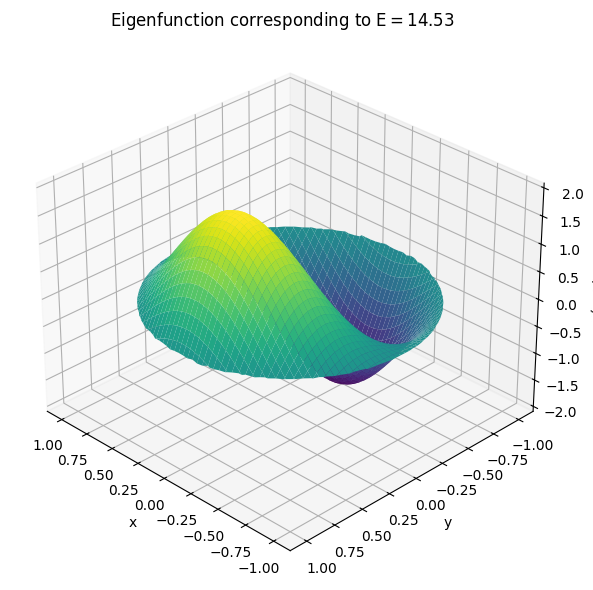
\includegraphics[width=.2\columnwidth]{eigen2-2.png} \\
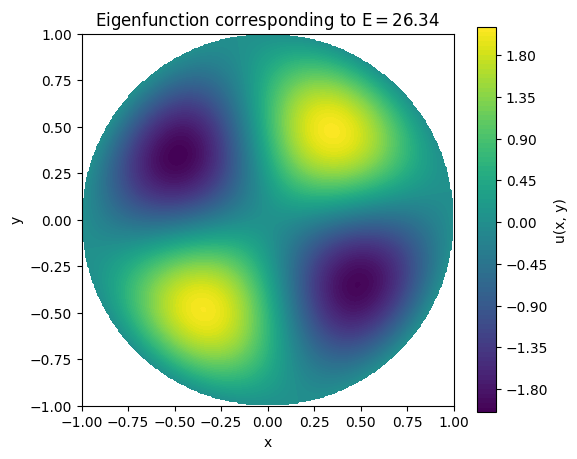
\includegraphics[width=.2\columnwidth]{eigen3-1.png} & 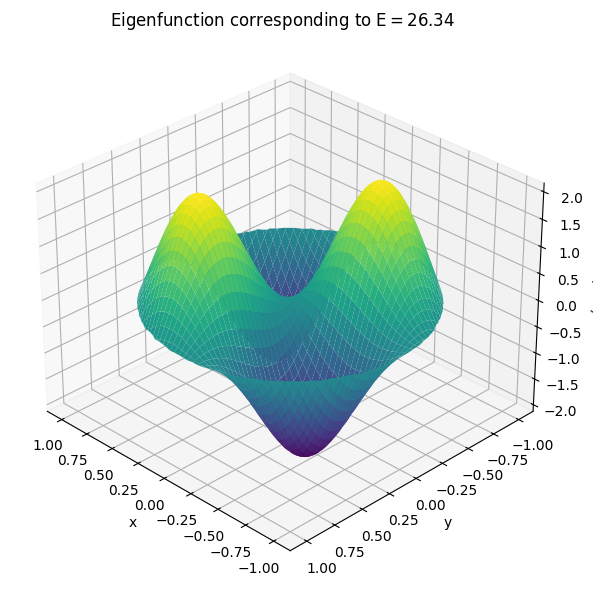
\includegraphics[width=.2\columnwidth]{eigen3-2.png} &
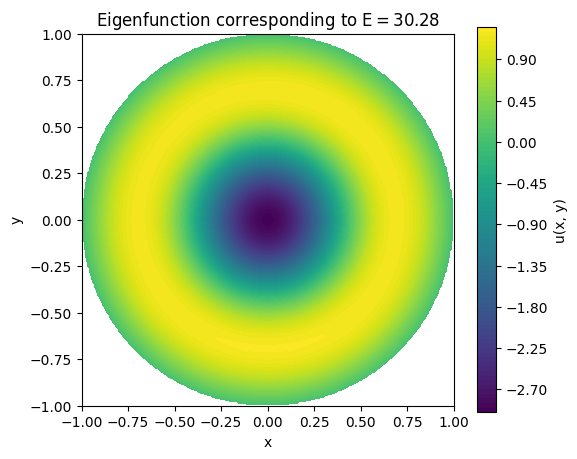
\includegraphics[width=.2\columnwidth]{eigen4-1.png} & 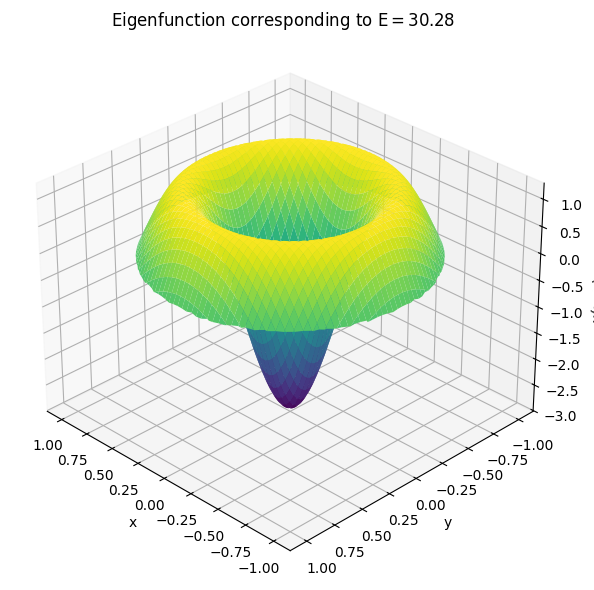
\includegraphics[width=.2\columnwidth]{eigen4-2.png} \\
\end{tabular}
\caption{The first four computed eigenfunctions of \eqref{eigen2} in the \rev{two-dimensional} unit disk.}
\label{func.fig}
\end{figure}

\subsection{Refinement and a posteriori certificate}\label{sec.certificate}
\begin{revblock}
Let $L=-\Delta+V$ and, for $u\in D(L)\setminus\{0\}$ (for instance a trained network),
\[
r(u,E)=\frac{\|(L-E)u\|_2}{\|u\|_2}=\Lambda(u,E)^{1/2},\qquad
\rho(u)=\frac{\langle Lu,u\rangle}{\|u\|_2^2},\qquad \eta(u)=r(u,\rho(u)).
\]

\begin{proposition}\label{prop.rayleigh}
Let $u\in D(L)\setminus\{0\}$. Then:
\begin{enumerate}
\item[(a)] $\Lambda(u,E)=(E-\rho(u))^2+\eta(u)^2$ for every $E\in\R$; in particular, for fixed $u$ the
minimum of $E\mapsto\Lambda(u,E)$ is attained at the Rayleigh quotient $\rho(u)$.
\item[(b)] (Weinstein \cite{Weinstein1934,Parlett1998}) $d(E)\le r(u,E)$ for every $E$: the interval
$[E-r,E+r]$ contains an eigenvalue of $L$.
\item[(c)] (Kato--Temple \cite{Kato1949,Parlett1998}) If $E_k$ is the only eigenvalue of $L$ in
$(\rho(u)-\gamma,\rho(u)+\gamma)$, then $|\rho(u)-E_k|\le\eta(u)^2/\gamma$.
\end{enumerate}
\end{proposition}

\noindent\emph{Refinement.} Once a local minimum $E^{i_0}$ of the discrete curve is detected, the
network $u^{i_0}$ is kept fixed and the eigenvalue is taken as the minimizer of
$E\mapsto\Lambda(u^{i_0},E)$, which by (a) is the Rayleigh quotient
\[
\hat E=\rho(u^{i_0})=-\frac{\int_\Omega u^{i_0}(\Delta u^{i_0}-Vu^{i_0})\,dx}{\int_\Omega (u^{i_0})^2\,dx}.
\]
No further training is needed. In the previous version of this paper this minimizer was computed
by a bounded scalar minimization of the Monte Carlo objective, re-sampled at every evaluation; a
stochastic objective of this kind is flat to within its noise, and the returned value has an error
of order the square root of the noise level. Evaluating the closed form on a fixed sample is both
cheaper and more accurate: on 14 minima detected in the unit square the median absolute error was
$6.6\times10^{-3}$ with the re-sampled minimization, $1.1\times10^{-3}$ with the closed form on
$10^5$ fixed Monte Carlo points and $6.6\times10^{-4}$ on a $300\times300$ midpoint grid (maximal
errors $1.3\times10^{-1}$, $5.5\times10^{-3}$, $5.8\times10^{-3}$); a three-point parabolic fit of the
loss values at coarse nodes was not reliable (median $9.7\times10^{-3}$, maximum $1.0$), because
different nodes carry different training floors. Table~\ref{table.1} and the tables of
Sections~\ref{sec.fem} and \ref{sec.nolin} use the closed form; Tables~\ref{table.2}--\ref{table.4}
are those of the previous version (re-sampled minimization).

\noindent\emph{Certificate.} Items (b) and (c) hold for \emph{any} $u\in D(L)$, whatever the quality
of the training. Hence each detected pair comes with the guaranteed enclosure
$|E-E_k|\le r$ (with $r=\mathrm{Residual}^{1/2}$, \emph{not} the Residual itself) and, if $\gamma$ is a
lower bound for the distance to the rest of the spectrum (obtainable from the enclosures of the
neighbouring detections), with $|\hat E-E_k|\le\eta^2/\gamma$. The eigenvalue error is therefore
\emph{quadratic} in the residual: a residual $\eta^2=10^{-1}$ and a gap $\gamma=10$ guarantee an
error at most $10^{-2}$, although $\eta\approx0.32$. This explains quantitatively the pattern
observed in all our tables, accurate eigenvalues together with comparatively large residuals. The
integrals in $r$ and $\rho$ are evaluated by Monte Carlo on fresh points, so the certificate is
statistical: the estimator of $\Lambda(u,E)$ has a bias $O(1/N)$ and a standard deviation
$O(N^{-1/2})$ that can be estimated from the same sample.
\end{revblock}

\noindent\rev{For the nonlinear problems of Section~\ref{sec.nolin} no analogue of the Weinstein or
Kato--Temple bounds is available; see Remark~\ref{rem.plap.lost}.}

\section{Further examples}\label{sec.examples}

In this section, we illustrate the flexibility of our method by applying it to a variety of settings beyond the two-dimensional unit disk with \rev{the hard-wall} potential. These examples include the computation of higher-order eigenvalues, problems in higher spatial dimensions, domains with different geometries, and more general potential functions.

\rev{The code is available in the repository given in the Declarations; it contains the scripts of
all the new experiments of this version (Table~\ref{table.1}, Sections~\ref{sec.fem},
\ref{sec.nolin} and \ref{sec.analysis}).}

\subsection{Higher eigenvalues}
Our method enables the computation of higher-order eigenvalues without relying on sequential orthogonalization procedures. By choosing an appropriate interval $[E_*, E^*]$, we can directly \rev{target} eigenvalues that are far from the principal one \rev{(in the examples below, up to the fourth eigenvalue $17\pi^2$ of the triangle, and the seventh distinct eigenvalue of the ball of $\R^3$, which is the 21st to 29th eigenvalue counted with multiplicity)}.

\rev{The choice of the penalty parameter $\mu$ in \eqref{lossmu} is discussed in Section~\ref{sec.mu}, where the heuristic $\mu\propto E^2$ of the previous version is replaced by a rule derived from Proposition~\ref{prop.penalized}: $\mu$ must exceed the square of the largest distance from the window to the spectrum, and a larger value of order $E^2/2$ is needed only when the network is trained from scratch at a high value of $E$.}

To assess the accuracy of our method, we computed the eigenvalues of problem \eqref{eigen2} in the two-dimensional unit square $[0,1]\times[0,1]$ that lie within the interval \rev{$[44, 55]$}. In this case we have taken $\mu=3000$. In this range, problem \eqref{eigen2} has one \rev{(double)} eigenvalue, \rev{$E_{(1,2)}=5\pi^2\approx49.348$}. See Fig.~\ref{eigen55.fig} for the computed loss curve in this interval, together with the \rev{exact curve}.

\rev{We also computed the eigenvalues of \eqref{eigen2} in the unit square in the window $[0,105]$
(80 grid points, $\mu=500$, at most 5000 epochs, re-initialization every 25 grid points).} In Table \ref{table.1} we compare the exact eigenvalues with those obtained by our method, together with the relative error and residuals. In Figures \ref{loss.lap.square.fig} and \ref{loss.lap.square.fig.2} we display the loss curve $\bar \Lambda (E)$ alongside the \rev{exact curve}, as well as the first two eigenfunctions.

\begin{figure}[htbp]
\centering
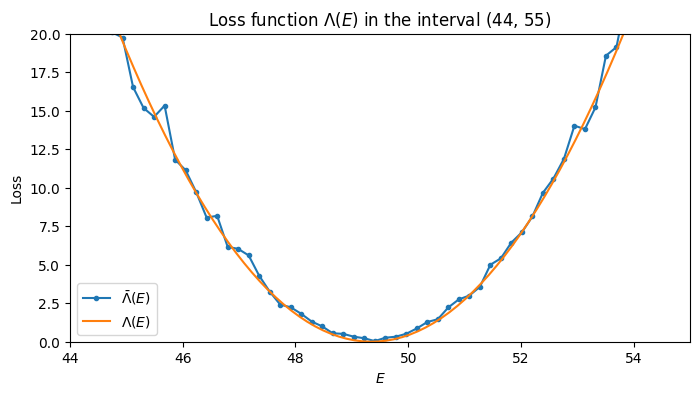
\includegraphics[width=.6\columnwidth]{loss_2d_cuadrado_entre_45_y_55_1er_autovalor.png}
\caption{The loss curve $\bar\Lambda(E)$ in the unit square computed in the interval \rev{$[44,55]$}.}
\label{eigen55.fig}
\end{figure}

\begin{table}[htbp]
\centering\small
\color{blue}
\caption{Eigenvalues of problem \eqref{eigen2} in the unit square $[0,1]\times[0,1]$ compared with the exact values (re-computed for this version; scan of $[0,105]$ with 80 nodes, $\mu=500$; $E$ is the Rayleigh quotient of the trained network evaluated on a $300\times300$ midpoint grid; Residual is evaluated on a fresh Monte Carlo sample at the reported $E$; $r=(\mathrm{Residual}/\overline{u^2})^{1/2}$ is the Weinstein radius). The double eigenvalues $5\pi^2$ and $10\pi^2$ appear as a single minimum; the multiplicity is not detected by the method.}
\label{table.1}
\begin{tabular}{cccccccc}
\toprule
$(m,n)$ & mult. & $E_{(m,n)}=\pi^2(m^2+n^2)$ & Our method & Rel.\ error & Residual & $r$ \\
\midrule
$(1,1)$ & 1 & $2\pi^2\approx 19.7392$ & 19.739909 & $3.5\times10^{-5}$ & $9.7\times10^{-2}$ & 0.31\\
$(1,2),(2,1)$ & 2 & $5\pi^2\approx 49.3480$ & 49.348167 & $2.9\times10^{-6}$ & $7.3\times10^{-2}$ & 0.27\\
$(2,2)$ & 1 & $8\pi^2\approx 78.9568$ & 78.956161 & $8.5\times10^{-6}$ & $2.0\times10^{-1}$ & 0.44\\
$(1,3),(3,1)$ & 2 & $10\pi^2\approx 98.6960$ & 98.695973 & $7.2\times10^{-7}$ & $9.3\times10^{-2}$ & 0.30\\
\bottomrule
\end{tabular}
\end{table}

\noindent\rev{In the previous version the row $(1,3)$ reported the value $98.594123$ with Residual
$1.40\times10^{-3}$, which is incompatible with the Weinstein bound ($|E-10\pi^2|=0.10>r=0.037$); that
row has been replaced by the re-computed one, and the whole table was re-run with the closed-form
refinement. In the new run all rows satisfy the Weinstein bound, with errors two to four orders
of magnitude below $r$.}

\begin{figure}[htbp]
\centering
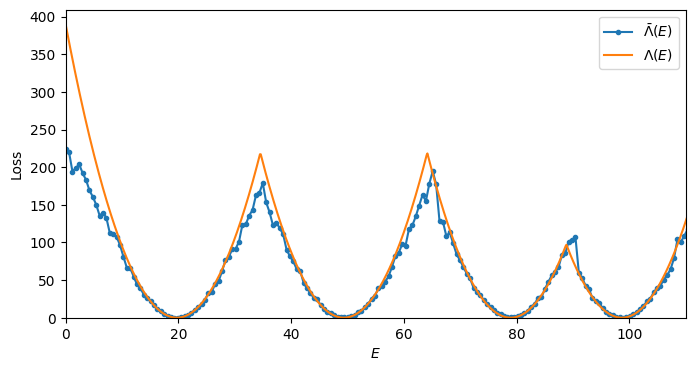
\includegraphics[width=.7\columnwidth]{loss_n=2_p=2_V=0_mu=450_cuadrado.png}
\caption{The loss curve $\bar\Lambda(E)$ in the unit square compared with the \rev{exact curve (run of the previous version, $\mu=450$)}.}
\label{loss.lap.square.fig}
\end{figure}

\begin{figure}[htbp]
\centering
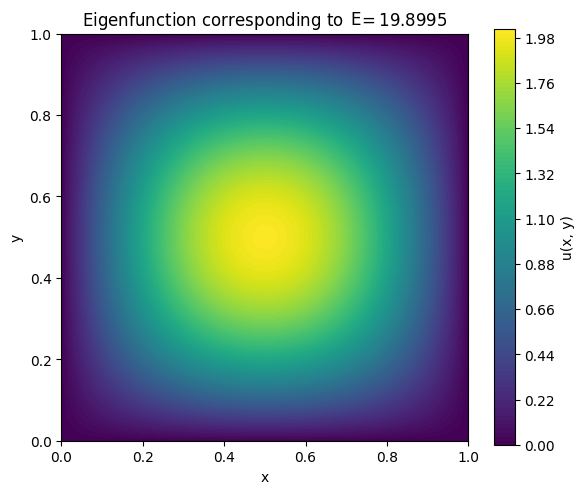
\includegraphics[width=.23\columnwidth]{n=2_p=2_v=0_mu=150_cuadrado_autof1.png}
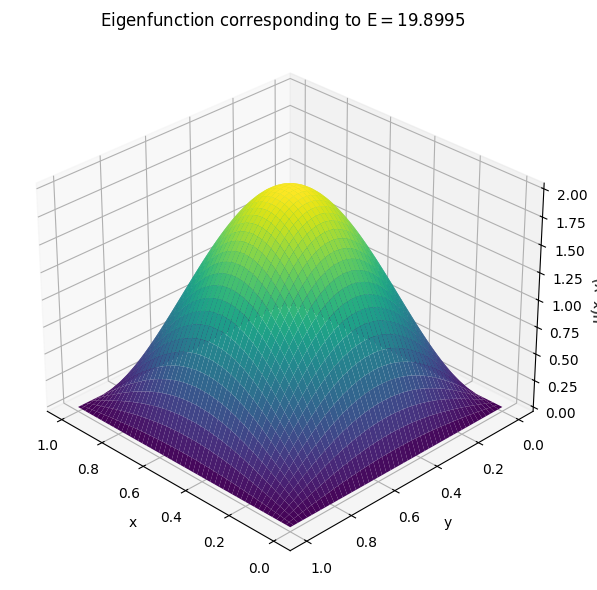
\includegraphics[width=.23\columnwidth]{n=2_p=2_v=0_mu=150_cuadrado_autof13d.png}
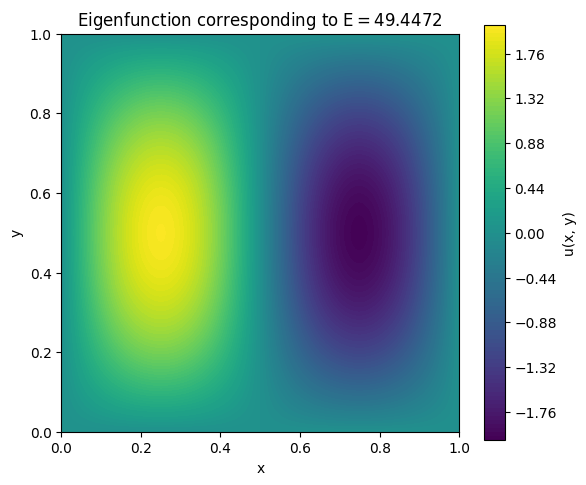
\includegraphics[width=.23\columnwidth]{n=2_p=2_v=0_mu=150_cuadrado_autof2.png}
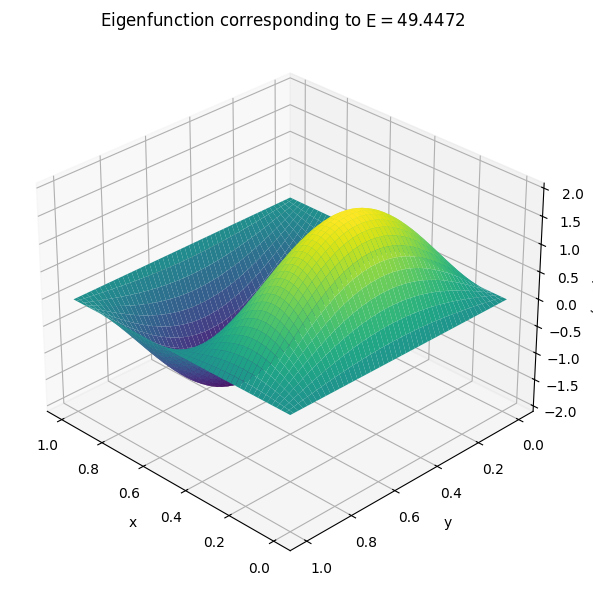
\includegraphics[width=.23\columnwidth]{n=2_p=2_v=0_mu=150_cuadrado_autof23d.png}
\caption{The first two computed eigenfunctions in the unit square.}
\label{loss.lap.square.fig.2}
\end{figure}


\subsection{Higher dimensions}

The proposed framework extends naturally to higher spatial dimensions, with minimal changes required in the implementation. As an example, we consider the unit ball in $\R^d$, with $d=3,4$\rev{,} where the eigenvalue problem becomes:
$$
\begin{cases}
-\Delta u = Eu & \text{in } B^d\\
u=0 & \text{on }\partial B^d.
\end{cases}
$$
Despite the increased computational cost, the method remains effective, as shown in Fig.~\ref{loss3D.fig}. In this example we considered \rev{$\mu=100$ for $d=3$ and $\mu=200$ for $d=4$}.

\rev{The eigenvalues are known explicitly: for $m\in\N_0$, $n\in\N$, $E_{(m,n)}=j_{m+\frac12,n}^2$ with multiplicity $2m+1$ if $d=3$, and $E_{(m,n)}=j_{m+1,n}^2$ with multiplicity $(m+1)^2$ if $d=4$, where $j_{\nu,n}$ is the $n$-th positive zero of the Bessel function $J_\nu$.}

In Tables \ref{table.2} and \ref{table.3}, we compare the exact eigenvalues with those obtained by our method.

\begin{table}[htbp]
\centering\small
\caption{Eigenvalues of problem \eqref{eigen2} in the unit ball in $\R^3$ compared with the exact values\rev{; $r=\mathrm{Residual}^{1/2}$ is the Weinstein radius}.}
\label{table.2}
\begin{tabular}{ccccccc}
\toprule
$(m,n)$ & \rev{mult.} & $E_{(m,n)} = j_{m+\frac12,n}^2$ & Our method & Relative error   & Residual & \rev{$r$} \\
\midrule
$(0,1)$ & \rev{1} & $\approx 9.8696$ & 9.885022 & $1.56\times 10^{-3}$ & $8.61\times 10^{-2}$ & \rev{0.29}\\
$(1,1)$ & \rev{3} & $\approx 20.1907$ & 20.182569 & $4.04\times 10^{-4}$ & $4.59\times 10^{-2}$ & \rev{0.21}\\
$(2,1)$ & \rev{5} & $\approx 33.2175$ & 33.243410 & $7.81\times 10^{-4}$ & $1.00\times 10^{-1}$ & \rev{0.32}\\
$(0,2)$ & \rev{1} & $\approx 39.4784$ & 39.494155 & $3.99\times 10^{-4}$ & $1.81\times 10^{-1}$ & \rev{0.43}\\
$(3,1)$ & \rev{7} & $\approx 48.8312$ & 48.826976 & $8.64\times 10^{-5}$ & $2.24\times 10^{-1}$ & \rev{0.47}\\
$(1,2)$ & \rev{3} & $\approx 59.6795$ & 59.734069 & $9.14\times 10^{-4}$ & $2.04\times 10^{-1}$ & \rev{0.45}\\
$(4,1)$ & \rev{9} & $\approx 66.9543$ & 66.991853 & $5.61\times 10^{-4}$ & $4.82\times 10^{-1}$ & \rev{0.69}\\
\bottomrule
\end{tabular}
\end{table}

\begin{table}[htbp]
\centering\small
\caption{Eigenvalues of problem \eqref{eigen2} in the unit ball in $\R^4$ compared \rev{with} the exact values\rev{; $r=\mathrm{Residual}^{1/2}$}.}
\label{table.3}
\begin{tabular}{ccccccc}
\toprule
$(m,n)$ & \rev{mult.} & $E_{(m,n)} = j_{m+1,n}^2$ & Our method & Relative error   & Residual & \rev{$r$}\\
\midrule
$(0,1)$ & \rev{1} & $\approx \rev{14.6820}$ & 14.641796 & $\rev{2.74}\times 10^{-3}$ & $3.84\times 10^{-3}$ & \rev{0.06}\\% TODO: v2/rev-2 gave 3.84e-2 for this residual; authors to confirm from the run logs
$(1,1)$ & \rev{4} & $\approx 26.3746$ & 26.257056 & $\rev{4.46}\times 10^{-3}$& $2.13\times 10^{-1}$ & \rev{0.46}\\
$(2,1)$ & \rev{9} & $\approx \rev{40.7065}$ & 40.794700 & $\rev{2.17}\times 10^{-3}$& $1.98\times 10^{-1}$ & \rev{0.45}\\
$(0,2)$ & \rev{1} & $\approx \rev{49.2185}$  & 49.175395  & $\rev{8.75}\times 10^{-4}$& $6.04\times 10^{-1}$ & \rev{0.78}\\
\bottomrule
\end{tabular}
\end{table}

\begin{figure}[htbp]
\centering
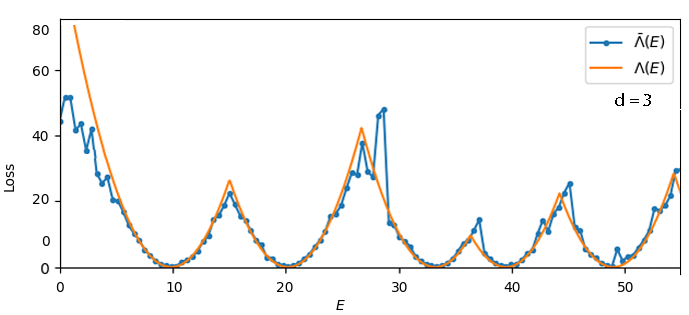
\includegraphics[width=.48\columnwidth]{loss_n=3_V=0_p=2_mu=100_reseteo_cada_15_iteraciones.png}
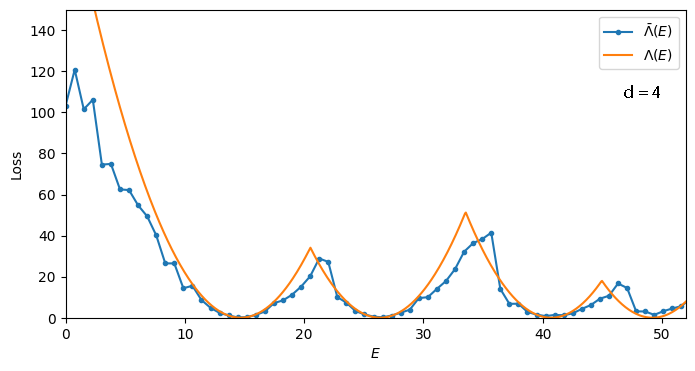
\includegraphics[width=.48\columnwidth]{loss_n=4_p=2_V=0_mu=200.png}
\caption{The loss curve $\bar\Lambda(E)$ in the unit ball of $\R^3$ \rev{(left)} and of $\R^4$ \rev{(right)} compared with the \rev{exact curve}.}
\label{loss3D.fig}
\end{figure}


\subsection{Different geometries}
We also explore \rev{other geometries: squares, annuli and triangles}. The boundary factor $B(x)$ \rev{(Section~\ref{sec.implementation})} is adapted to these shapes, ensuring that the Dirichlet condition is enforced. In Fig.~\ref{loss.lap.square.fig.2}, we show eigenfunctions obtained in a square, in Fig.~\ref{loss.lap.annulus.fig}  the annular region is considered and in \rev{Figs.}~\ref{loss.lap.triang.fig} and \ref{loss.lap.triang.fig.2} the results in \rev{the triangle with vertices $(0,0)$, $(1,0)$, $(0,1)$} are shown. In that example we considered $\mu=15000$ \rev{(window $[0,180]$)}.

In Table \ref{table.4}, the exact eigenvalues of \eqref{eigen2} in \rev{this} triangle are compared with those obtained by our method. \rev{The Dirichlet eigenfunctions of the triangle are $\sin(m\pi x_1)\sin(n\pi x_2)-(-1)^{m+n}\sin(n\pi x_1)\sin(m\pi x_2)$, $m>n\ge1$, with eigenvalue $\pi^2(m^2+n^2)$; all the eigenvalues in the window are simple (the previous version listed each of them twice).}

\begin{table}[htbp]
\centering\small
\caption{Eigenvalues of problem \eqref{eigen2} in the triangle with vertices $(0,0)$, \rev{$(1,0)$, $(0,1)$} compared with the exact values. \rev{All the eigenvalues listed are simple; these are all the eigenvalues in $[0,180]$; $r=\mathrm{Residual}^{1/2}$.}}
\label{table.4}
\begin{tabular}{cccccc}
\toprule
$(m,n)$ & $E_{(m,n)} = \pi^2 (m^2 + n^2)$ & Our method & Relative error  & Residual & \rev{$r$}\\
\midrule
$(2,1)$ & $5\pi^2\approx \rev{49.3480}$   & 49.369942  & $4.44\times 10^{-4}$ & $2.42\times 10^{-1}$ & \rev{0.49}\\
$(3,1)$ & $10\pi^2\approx \rev{98.6960}$  & 98.892161  & $1.99\times 10^{-3}$ & $1.26$ & \rev{1.12}\\
$(3,2)$ & $13\pi^2\approx 128.3049$ & 128.048509 & $2.00\times 10^{-3}$ & $1.98$ & \rev{1.41}\\
$(4,1)$ & $17\pi^2\approx 167.7833$ & 167.687185 & $5.73\times 10^{-4}$ & $2.16$ & \rev{1.47}\\
\bottomrule
\end{tabular}
\end{table}

\begin{figure}[htbp]
\centering
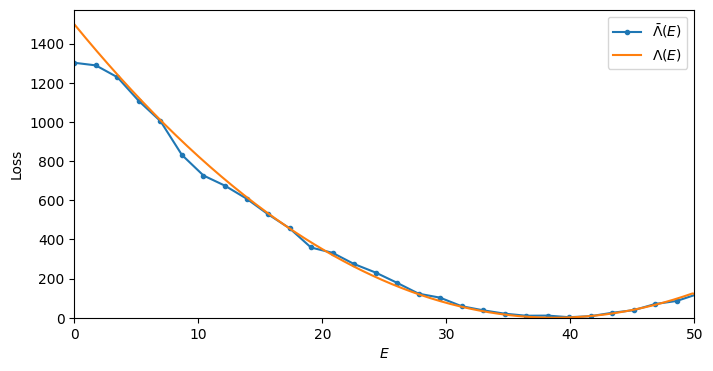
\includegraphics[width=.3\columnwidth]{loss_n=2_p=2_V=0_annulus.png}
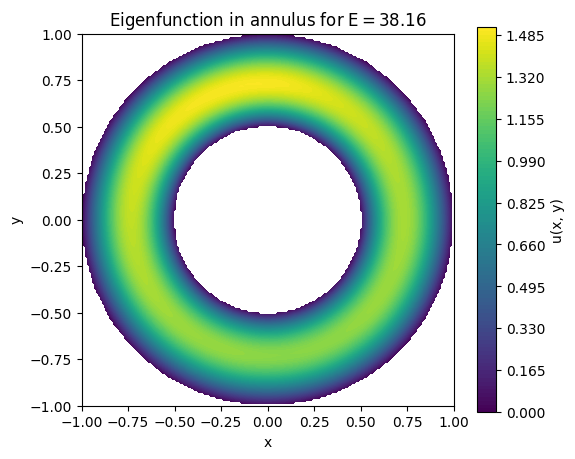
\includegraphics[width=.3\columnwidth]{eigen1-annulus.png}
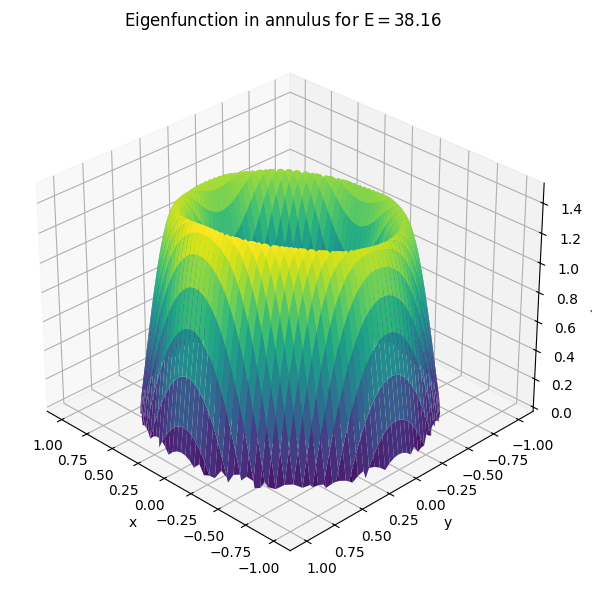
\includegraphics[width=.3\columnwidth]{eigen1-3d-annulus.png}
\caption{\rev{Left: the loss curve $\bar\Lambda(E)$ in the annulus $\{0.5<|x|<1\}$; the reference curve drawn in this plot (previous version) contains only the first eigenvalue $39.0133$, whereas the window also contains $40.8725$ (double) and $46.4285$ (double). The PINN scan followed the radial branch and missed these two eigenvalues (an example of a missed eigenvalue, see Section~\ref{sec.stability}). Centre and right: the first computed eigenfunction.}}
\label{loss.lap.annulus.fig}
\end{figure}

\begin{figure}[htbp]
\centering
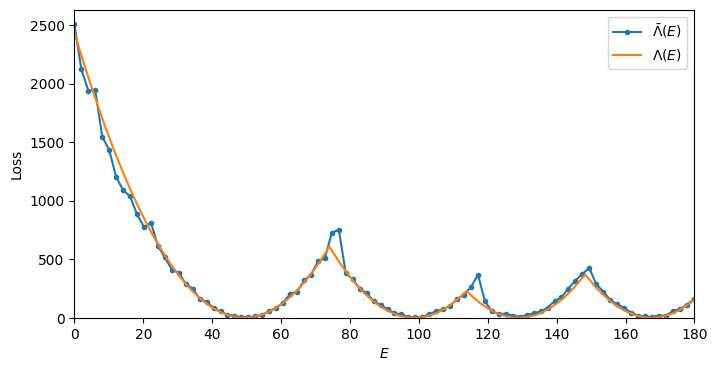
\includegraphics[width=.7\columnwidth]{loss_n=2_p=2_V=0_mu=15000_triangulo.png}
\caption{The loss curve $\bar\Lambda(E)$ in the triangle \rev{with} vertices $(0,0)$, $(0,1)$, $(1,0)$ compared with the \rev{exact curve}.}
\label{loss.lap.triang.fig}
\end{figure}

\begin{figure}[htbp]
\centering
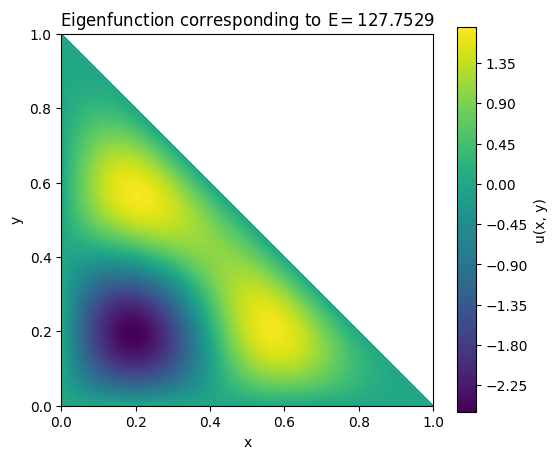
\includegraphics[width=.24\columnwidth]{eigen_p=2_n=2_V=0_triangulo_4.png}
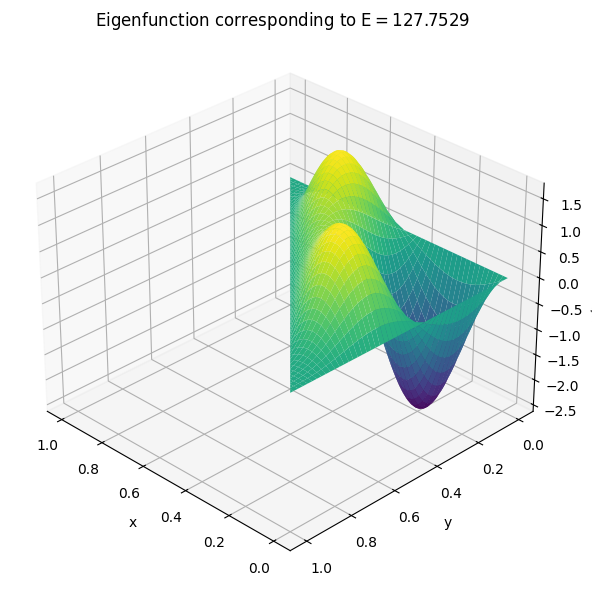
\includegraphics[width=.24\columnwidth]{eigen_p=2_n=2_V=0_triangulo_4_3d.png}
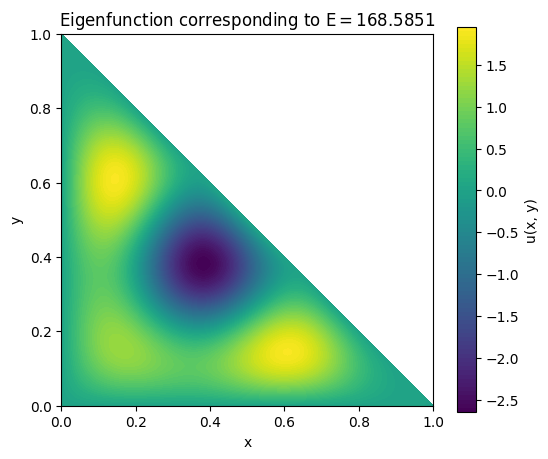
\includegraphics[width=.24\columnwidth]{eigen_p=2_n=2_V=0_triangulo_5.png}
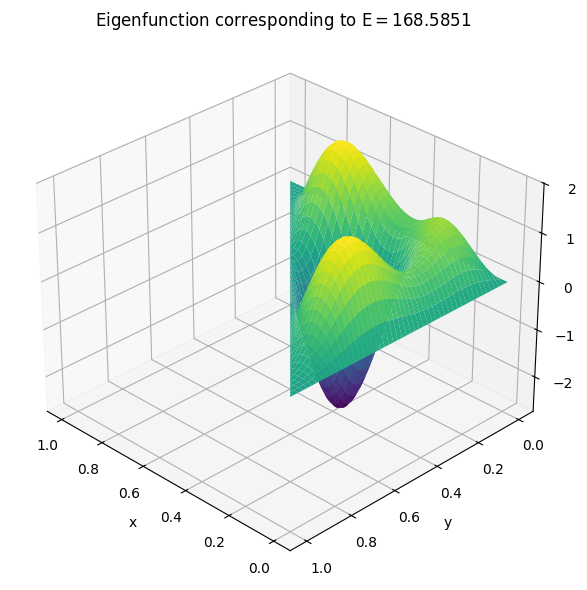
\includegraphics[width=.24\columnwidth]{eigen_p=2_n=2_V=0_triangulo_5_3d.png}
\caption{Third and fourth computed eigenfunctions in the triangle \rev{with} vertices $(0,0)$, $(0,1)$, $(1,0)$ \rev{(from a different run than Table~\ref{table.4}; the panel titles show the values of that run)}.}
\label{loss.lap.triang.fig.2}
\end{figure}


\subsection{Different potentials}\label{sec.potentials}

Beyond hard-wall confinement, our approach accommodates general potential functions $V(x)$\rev{; the problem is always solved in the unit disk or ball with Dirichlet boundary condition}.

As an example, we consider a harmonic potential $V(x)=\frac{\omega^2}{2}|x|^2$ \rev{in the unit disk} for different values of $\omega$\rev{; note that, because of the boundary condition, this is not the harmonic oscillator on $\R^2$}. Fig.~\ref{pot2.fig} displays \rev{the} loss curve and the first eigenfunction for $\omega=1$ and Fig.~\ref{pot1.fig} for $\omega=10$. In Fig.~\ref{fig.well-two}, we display the double-well Gaussian potential \rev{in the unit ball of $\R^3$,
\[
V(x)=-V_0\Big(e^{-|x-ae_1|^2/(2\sigma^2)}+e^{-|x+ae_1|^2/(2\sigma^2)}\Big),\qquad a=1,\ \sigma=0.5,\ V_0=1,
\]
i.e.\ $V(x)=-e^{-2|x-x_0|^2}-e^{-2|x+x_0|^2}$ with $x_0=e_1=(1,0,0)$; the centres of the wells lie on the boundary sphere,} together with the loss curve.

Finally, in Fig.~\ref{fig.well-four} we consider a four-well compactly supported potential \rev{in the unit ball of $\R^3$} and we plot the corresponding loss curve. More precisely, \rev{for $x\in\R^3$ let} the centers of the four wells \rev{be} $c_1 = (a,a,0)$, $c_2 = (-a,a,0)$, $c_3 = (a,-a,0)$, $c_4 = (-a,-a,0)$, where $a=0.22$, \rev{let $\sigma=0.2$, and} define the compactly supported bump function
$$
\phi(t) =
\begin{cases}
\exp(-(1-t^2)^{-1}), & t < 1,\\
0, & t \ge 1.
\end{cases}
$$
Then the potential is
$
V(x) = - \sum_{i=1}^{4} \phi\big( |x - c_i|/\sigma \big)
$
\rev{(depth $e^{-1}\approx0.37$ at each centre)}.

\rev{In the harmonic, double-well and four-well examples we used $\mu=100$, $400$ and $1000$, respectively (2000 sampling points for the four-well potential).}

\begin{figure}[htbp]
\centering
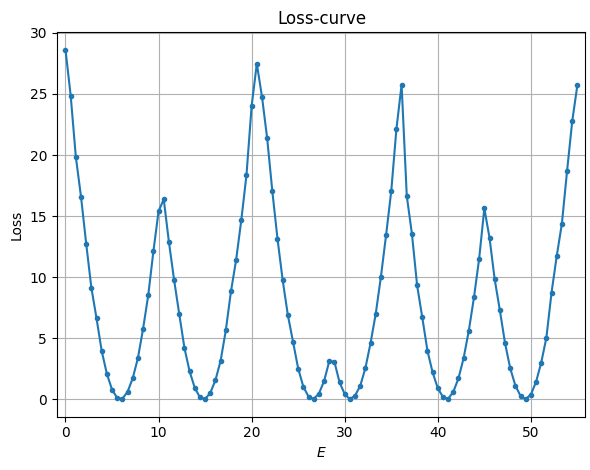
\includegraphics[width=.3\columnwidth]{loss_p=2_n=2_V=harmonic_omega=1_disco.png}
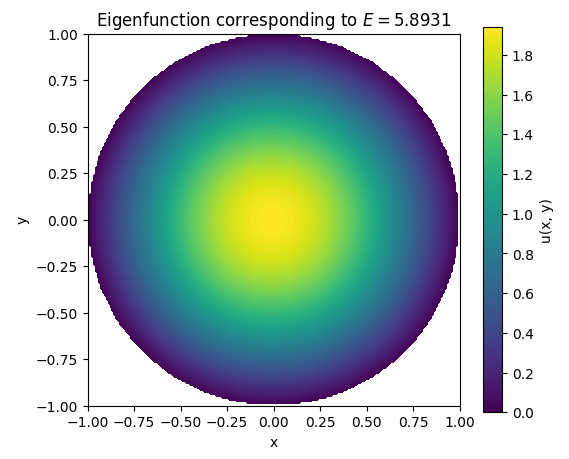
\includegraphics[width=.3\columnwidth]{egen_p=2_n=2_V=harmonic_omega=1_disco_1.png}
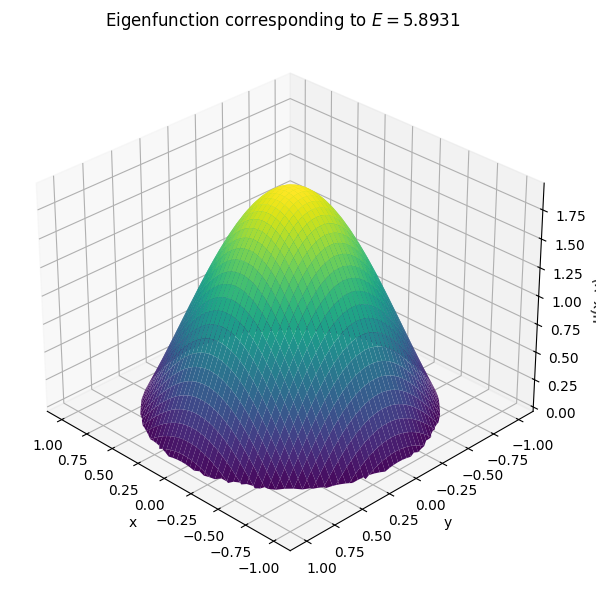
\includegraphics[width=.3\columnwidth]{egen_p=2_n=2_V=harmonic_omega=1_disco_1_3d.png}
\caption{The loss curve $\bar\Lambda(E)$ in the unit disk with harmonic potential $V=\frac{\omega^2}{2}|x|^2$ and $\omega=1$ with the first computed eigenfunction\rev{. The minima are at the eigenvalues $5.8919$, $14.8484$, $26.5790$, $30.6271$, $40.9385$, $49.3852$ (finite element reference, Section~\ref{sec.fem})}.}
\label{pot2.fig}
\end{figure}

\begin{figure}[htbp]
\centering
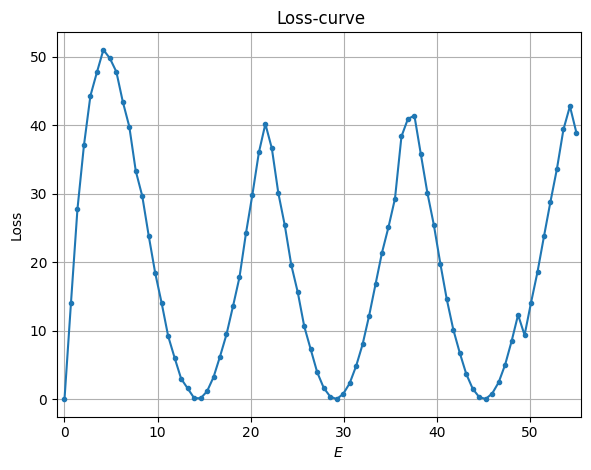
\includegraphics[width=.3\columnwidth]{loss_n=2_V=harmonic_p=2.png}
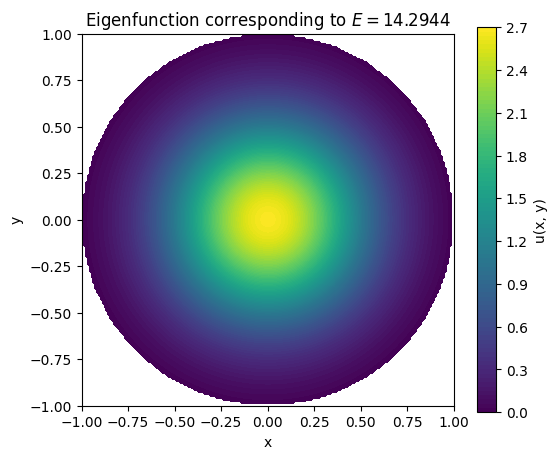
\includegraphics[width=.3\columnwidth]{eigen_n=2_V=harmonic_p=2_1.png}
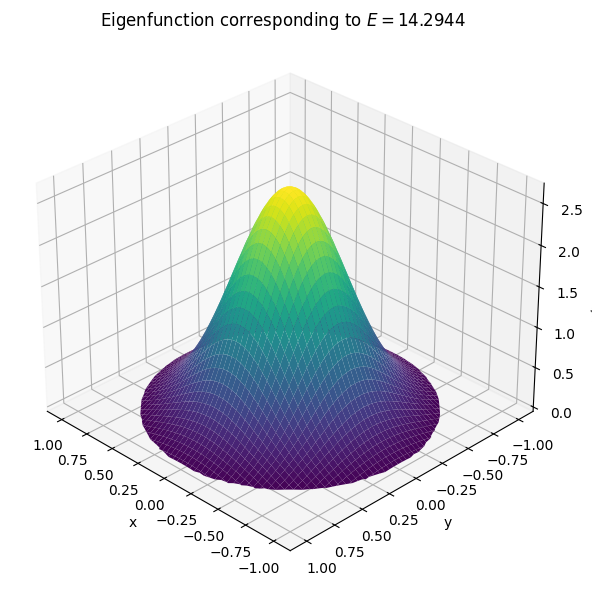
\includegraphics[width=.3\columnwidth]{eigen_n=2_V=harmonic_p=2_1_3d.png}
\caption{The loss curve $\bar\Lambda(E)$ in the unit disk with harmonic potential $V=\frac{\omega^2}{2}|x|^2$ and $\omega=10$ with the first computed eigenfunction\rev{. The eigenvalues in the window are $14.2847$, $29.1349$ (double), $45.0887$ (double), $46.2907$; the last two are $1.2$ apart and appear as a single minimum (grid step $\approx0.7$). The value $\bar\Lambda=0$ at $E=0$ is the trivial state $u=0$ ($d(0)^2=204>2\mu=200$, Proposition~\ref{prop.penalized})}.}
\label{pot1.fig}
\end{figure}

\begin{figure}[htbp]
\centering
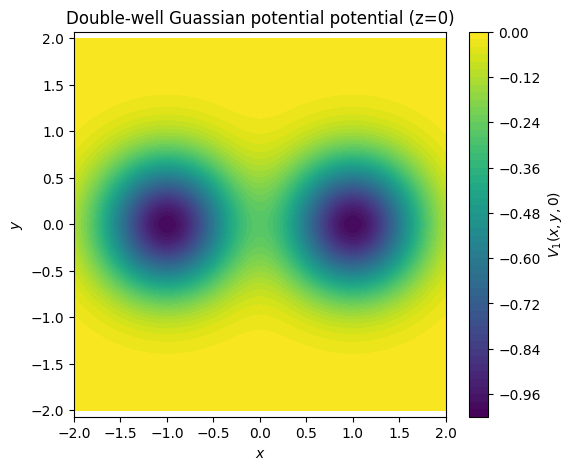
\includegraphics[width=.4\columnwidth]{well-1.png}
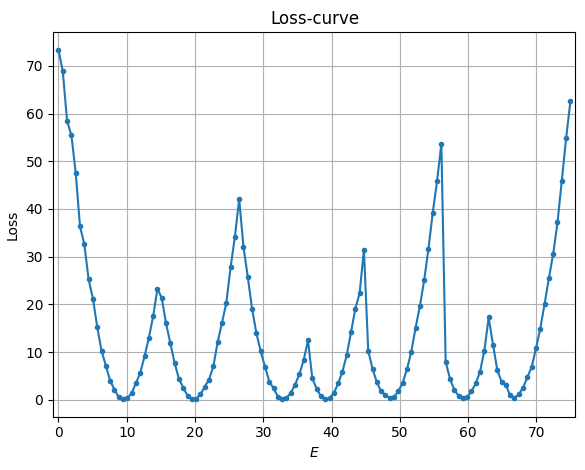
\includegraphics[width=.4\columnwidth]{well-1-plot.png}
\caption{\rev{Double-well Gaussian potential (left) and loss curve $\bar\Lambda(E)$ (right) in the unit ball of $\R^3$.}}
\label{fig.well-two}
\end{figure}

\begin{figure}[htbp]
\centering
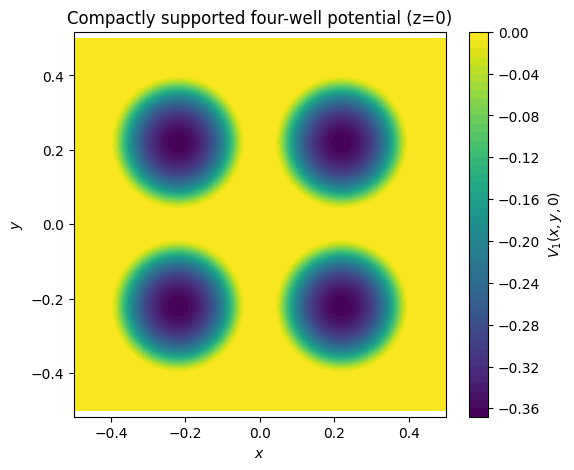
\includegraphics[width=.4\columnwidth]{well-2.png}
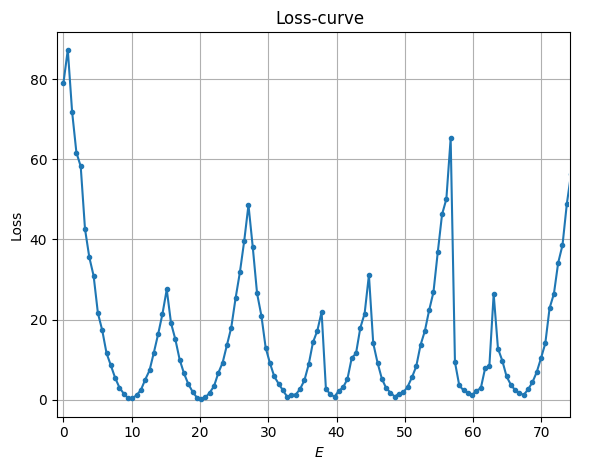
\includegraphics[width=.4\columnwidth]{well-2-plot.png}
\caption{\rev{Compactly supported four-well potential (left) and loss curve $\bar\Lambda(E)$ (right) in the unit ball of $\R^3$.}}
\label{fig.well-four}
\end{figure}

\subsection{Validation with the finite element method}\label{sec.fem}
\begin{revblock}
For the potentials no closed-form eigenvalues are available, so we computed independent reference
values with a finite element method: Lagrange $P_2$ elements on curved (isoparametric) meshes,
generalized eigenvalue problem solved by shift-invert Lanczos, Richardson extrapolation over the
last three uniform refinements. The finite element code reproduces the exact eigenvalues of the
disk, annulus, square and triangle with errors $10^{-10}$--$10^{-6}$ (observed order $4$ in two
dimensions) and those of the ball of $\R^3$ with errors $7\times10^{-5}$ to $1.6\times10^{-2}$
for $E\le67$ (observed order $\approx2.8$, three mesh levels with up to $41\,727$ degrees of
freedom); the reported uncertainty of the extrapolated values is conservative on these test cases.

For each potential we then trained the PINN on four windows of seven grid points (step $0.5$),
with the settings of Section~\ref{sec.potentials} and 2--3 seeds; the eigenvalue is the Rayleigh
quotient of the network at the node of smallest normalized loss. \emph{The windows were centred at
the finite element values}: this is a test of the accuracy of the loss curve at known eigenvalues,
not a blind detection. Table~\ref{table.fem} and Fig.~\ref{fig.fem} show the results.

\begin{table}[tbp]
\centering\small
\color{blue}
\caption{PINN versus finite elements (FEM) for the potentials of Section~\ref{sec.potentials}. FEM: extrapolated value of the nearest eigenvalue (multiplicity); $^\dagger$: other FEM eigenvalues within $0.75$, i.e.\ a cluster that the scan does not resolve. $\hat E$: Rayleigh quotient of the trained network, mean over seeds [min, max]. Rel.\ err.\ is with respect to the FEM value.}
\label{table.fem}
\begin{tabular}{lcccc}
\toprule
example & FEM (mult.) & $\hat E$ (PINN) & rel.\ err.\ (\%) & $\min\Lambda$\\
\midrule
double well, ball $\R^3$ & $9.5764$ (1) & 9.5782 [9.5782, 9.5783] & $+0.02$ & 0.065\\
 & $19.7522^\dagger$ (1) & 19.7593 [19.7547, 19.7640] & $+0.04$ & 0.077\\
 & $32.8735^\dagger$ (2) & 32.9062 [32.8571, 32.9552] & $+0.10$ & 0.117\\
 & $39.1924$ (1) & 39.1941 [39.1938, 39.1944] & $+0.004$ & 0.108\\
\midrule
four well, ball $\R^3$ & $9.8542$ (1) & 9.8606 [9.8581, 9.8646] & $+0.07$ & 0.355\\
 & $20.1801^\dagger$ (2) & 20.1751 [20.1505, 20.1878] & $-0.03$ & 0.478\\
 & $33.2104^\dagger$ (2) & 33.2093 [33.2061, 33.2141] & $-0.003$ & 0.407\\
 & $39.4573$ (1) & 39.4515 [39.4414, 39.4578] & $-0.02$ & 1.054\\
\midrule
harmonic $\omega=10$, disk & $14.2847$ (1) & 14.2901 [14.2899, 14.2904] & $+0.04$ & 0.174\\
 & $29.1349$ (2) & 29.1355 [29.1353, 29.1357] & $+0.002$ & 0.056\\
 & $45.0887$ (2) & 45.0892 [45.0892, 45.0892] & $+0.001$ & 0.065\\
 & $62.5793$ (2) & 62.5796 [62.5792, 62.5800] & $+0.0005$ & 0.076\\
\bottomrule
\end{tabular}
\end{table}

\begin{figure}[tbp]
\centering
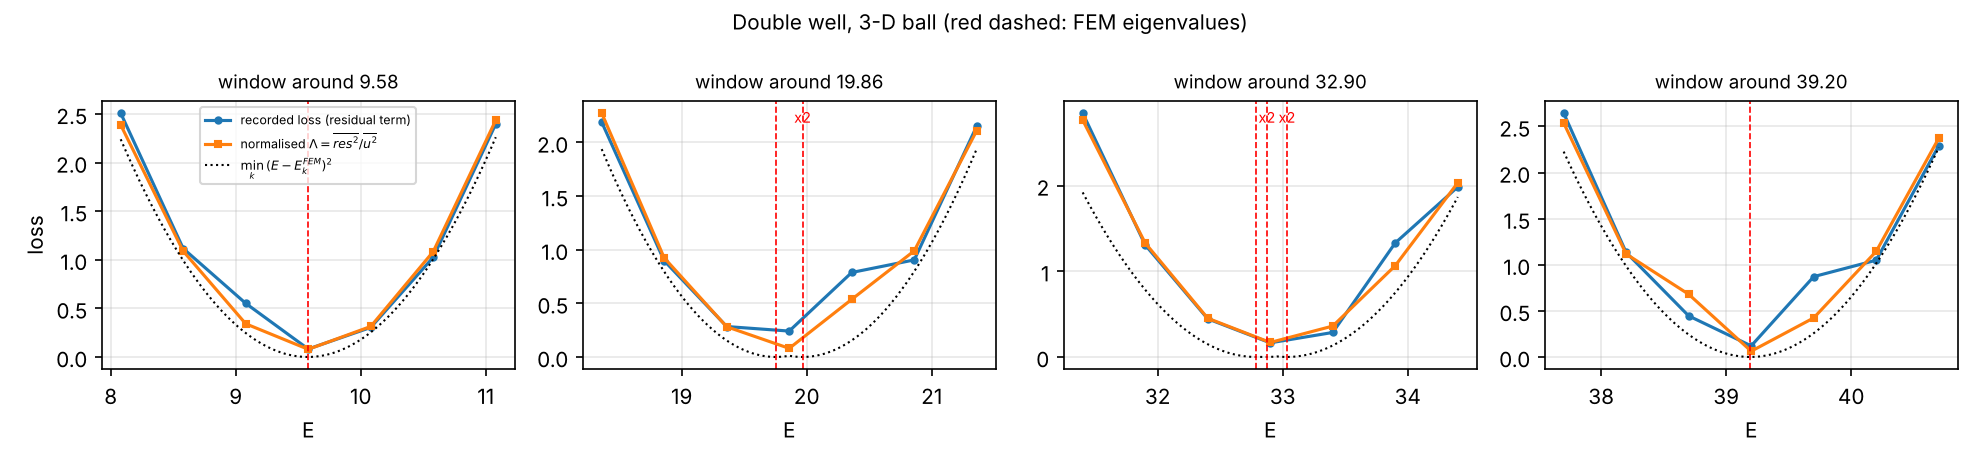
\includegraphics[width=.85\textwidth]{pinn_vs_fem_double_well.png}\\
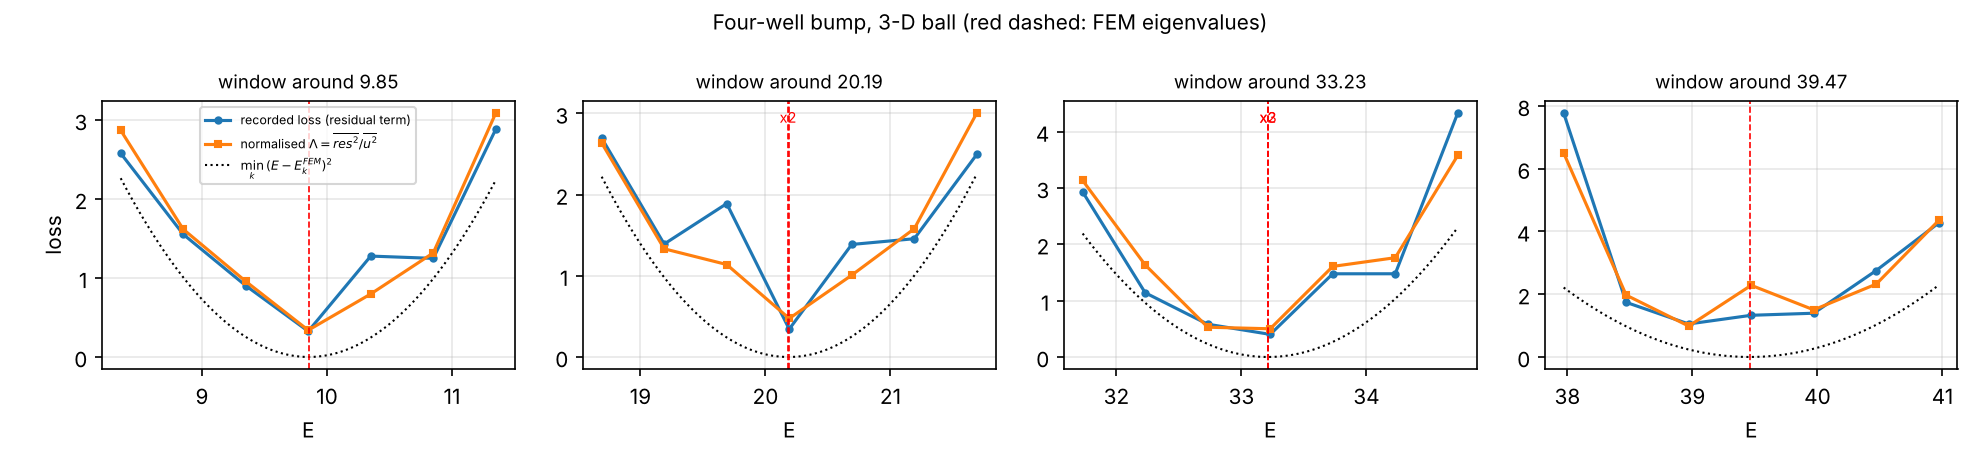
\includegraphics[width=.85\textwidth]{pinn_vs_fem_four_well.png}\\
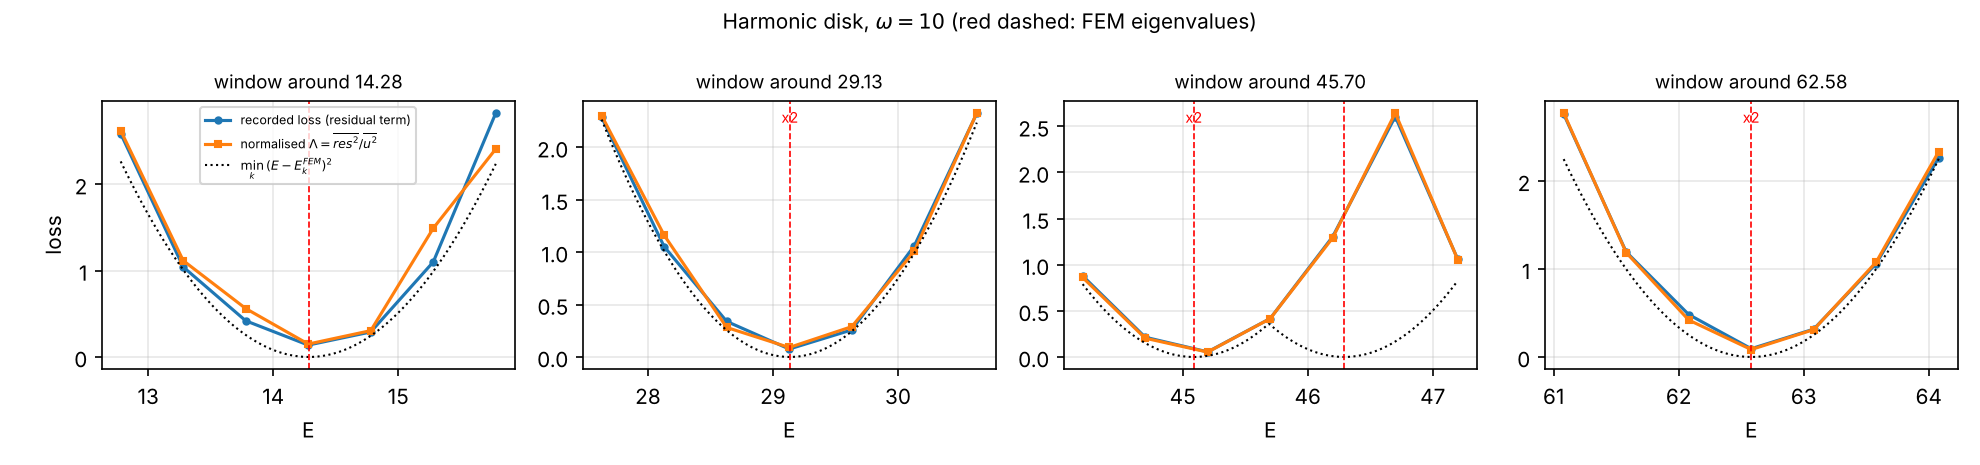
\includegraphics[width=.85\textwidth]{pinn_vs_fem_harm_w10.png}
\caption{PINN loss curves on windows centred at finite element eigenvalues (red dashed lines; ``x2'': double) for the double-well (top), four-well (middle) and harmonic $\omega=10$ (bottom) potentials: recorded residual term, normalized loss $\Lambda$, and $\min_k(E-E_k^{\rm FEM})^2$ (dotted).}
\label{fig.fem}
\end{figure}

The findings are the following. (i) In all windows the PINN eigenvalue agrees with the finite
element value to within $0.1\%$ (typically $10^{-4}$--$5\times10^{-4}$ in relative terms), although
the minimum of the loss is not zero ($\min\Lambda=0.06$--$1.05$, i.e.\ $r=0.25$--$1$): as explained in
Section~\ref{sec.certificate}, the accuracy comes from the Rayleigh quotient, whose error is
quadratic in $r$. (ii) The spectra of the well potentials consist of \emph{clusters of close
eigenvalues}: for the double well $19.75$ and $19.97$ (double), and $32.79$, $32.87$ (double),
$33.03$ (double); for the four well $20.180$ (double) and $20.189$, and $33.210$ (double) and
$33.214$ (triple). The loss curve has one minimum per cluster and the quotient returns a value
inside the cluster; the number of eigenvalues in the cluster and their multiplicities cannot be
read from the curve (see Remark~\ref{rem.stability}). (iii) The well potentials are weak perturbations
of the free ball: the first eigenvalue moves from $\pi^2=9.8696$ to $9.5764$ (double well) and to
$9.8542$ (four well); for the four-well potential the shift is of the same order as the PINN error,
so this example hardly distinguishes the potential from $V=0$. (iv) In the harmonic case with
$\omega=10$, the window around $45.7$ contains the double eigenvalue $45.0887$ and the simple
eigenvalue $46.2907$; the warm-started network stays on the branch of $45.09$ and the eigenvalue
$46.29$ is missed (gap $1.2$, step $0.5$), the same effect visible in Fig.~\ref{pot1.fig}.
(v) For these linear problems the finite element method is two to three orders of magnitude cheaper
and more accurate: a 7-point PINN window took $7$--$25$ minutes on one CPU core, whereas the finite
element computation of all eigenvalues in $[0,75]$ with multiplicities took less than $10$\,s in
two dimensions and about $2$ minutes for the ball of $\R^3$. As stated in Section~\ref{sec.approach},
the purpose of the method is not to compete with finite elements on linear problems.
\end{revblock}


\section{Nonlinear problems} \label{sec.nolin}

Our method can also be extended to nonlinear eigenvalue problems. As an illustrative example, we consider the eigenvalue problem for the $p$-Laplacian:
\begin{equation}\label{p-eigen}
\begin{cases}
-\nabla \cdot (|\nabla u|^{p-2} \nabla u) = E |u|^{p-2} u & \text{in } \rev{\Omega}, \\
u = 0 & \text{on } \partial \rev{\Omega},
\end{cases}
\end{equation}
where $\rev{\Omega} \subset \R^{\rev{d}}$ is \rev{a bounded domain} and $p > 1$.

To approximate the solution using our framework, we modify the loss function accordingly. For a fixed $E$, we define the following loss:
\begin{equation}\label{loss.p}
\bar\Lambda_p(u, E) = \int_{\rev{\Omega}} \left( \Delta_p u + E |u|^{p-2} u \right)^2 \, dx + \mu \left( \int_{\rev{\Omega}} |u|^p\, dx - 1 \right)^2,
\end{equation}
where $\Delta_p u = \nabla \cdot (|\nabla u|^{p-2} \nabla u)$\rev{, and the loss curve $\Lambda_p(E)=\inf_u\bar\Lambda_p(u,E)$}.

\begin{revblock}
\begin{remark}[Correction with respect to the previous version]\label{rem.correction}
The implementation used for the $p$-Laplacian results of the previous version of this paper did not
implement \eqref{loss.p}: the zero-order term of the residual was $E\,u$ instead of $E|u|^{p-2}u$,
and the normalization was $\int u^2=|\Omega|$ instead of $\int|u|^p=1$. The resulting equation
$-\Delta_pu=Eu$ is not homogeneous: if $(E,u)$ solves it, so does $(|t|^{p-2}E,tu)$, so the computed
value depended on the normalization and was not an eigenvalue of \eqref{p-eigen}. This explains the
errors of $2$--$7\%$ of the former Tables~5 and 6 (e.g.\ the former first eigenvalue of the disk,
$6.679$, lies between the true value $6.532$ and the value $6.935$ of the non-homogeneous problem) and
the former value $17.4513$ for the ball of $\R^3$, $p=2.5$, which is $24\%$ above the true first
eigenvalue $14.1112$ and within $1\%$ of the value $17.59$ of the non-homogeneous problem. Re-running
the former loss with our code gives $17.62$ in the ball and, in the disk, a flat and noisy curve between
$E=6.25$ and $7.25$ with frozen-network value $6.93$, which explains the former values. All the results of this section have been
recomputed with the loss \eqref{loss.p}; the former Tables~5--6 and Figs.~14--16 are replaced by
Tables~\ref{tab.plap}--\ref{tab.plap.p} and Fig.~\ref{fig.plap}.
\end{remark}
\end{revblock}

\begin{revblock}
\subsection{What can be proved}
For $p\ne2$ the eigenvalues of \eqref{p-eigen} form a closed set $\sigma_p\subset(0,\infty)$; the
first eigenvalue is simple and isolated \cite{Anane1987,Lindqvist1990}, there is a sequence of
variational (Lusternik--Schnirelmann) eigenvalues \cite{GarciaAzorero-Peral}, the second
eigenvalue coincides with the second variational one \cite{Anane-Tsouli} and has a mountain-pass
characterization \cite{Cuesta-deFigueiredo-Gossez}, which is the basis of the algorithm of
\cite{HJ11}. It is not known whether the variational eigenvalues exhaust $\sigma_p$. Eigenfunctions
are bounded and of class $C^{1,\alpha}$ \cite{DiBenedetto,Tolksdorf}, but in general not $C^2$.

\begin{proposition}\label{prop.plap}
Let $p>1$ with $p\ge\frac{2d}{d+2}$, and let $\mathcal D_p=\{u\in W^{1,p}_0(\Omega)\cap
L^{2(p-1)}(\Omega)\colon\Delta_pu\in L^2(\Omega)\}$. Then:
\begin{enumerate}
\item[(a)] If $u_k$ is an eigenfunction with eigenvalue $E_k$ and $\|u_k\|_p=1$, then
$\bar\Lambda_p(u_k,E)=c_k(E-E_k)^2$ with $c_k=\int_\Omega|u_k|^{2(p-1)}dx$; hence
$\Lambda_p(E)\le\inf_kc_k(E-E_k)^2$, the infimum being taken over all normalized eigenpairs.
\item[(b)] $\Lambda_p(E)=0$ if and only if $E\in\sigma_p$.
\end{enumerate}
\end{proposition}
The proof is given in Appendix~\ref{app.proofs}. Thus the zeros of the loss curve are exactly the
eigenvalues, without any orthogonality; this is the justification of the method for $p\ne2$.
For $p=2$, (a) reduces to the identity \eqref{cota.igual}.

\begin{remark}[What is lost with respect to the linear case]\label{rem.plap.lost}
(1) The proof of (b) is by compactness and gives no lower bound of the form
$\Lambda_p(E)\ge c\,\dist(E,\sigma_p)^2$: there is no analogue of the Weinstein bound, a small value
of the loss does not certify an eigenvalue, and a minimum with no independent reference is only a
candidate. (2) The constants $c_k$ depend on the eigenfunction, so the curvature of the wells is not
known a priori. (3) For fixed $u$, $E\mapsto\int(\Delta_pu+E|u|^{p-2}u)^2$ is still a parabola,
minimized at
\[
E_{\rm PINN}(u)=-\frac{\int_\Omega\Delta_pu\,|u|^{p-2}u\,dx}{\int_\Omega|u|^{2(p-1)}dx},
\]
which we use as the refined eigenvalue (the frozen-network refinement of
Section~\ref{sec.certificate}). For $p\ne2$ this is not the variational quotient
$\int|\nabla u|^p/\int|u|^p$, so its error is in general of first order in the error of the
eigenfunction (instead of second order for $p=2$).
\end{remark}

\begin{lemma}[Degeneracy at critical points]\label{lem.critical}
Let $p>2$, $u\in C^2$ near $x_0$ and $\nabla u(x_0)=0$. Then $\Delta_pu(x_0)=0$; hence the residual
of \eqref{p-eigen} at $x_0$ equals $E|u(x_0)|^{p-2}u(x_0)$, and an eigenfunction cannot be $C^2$ near
a critical point where it does not vanish.
\end{lemma}
\begin{proof}
For $p>2$, $\Phi(\xi)=|\xi|^{p-2}\xi$ is $C^1$ with $D\Phi(0)=0$, so $\Phi(\nabla u)$ is $C^1$ and
\[
\Delta_pu(x_0)=\operatorname{tr}\big(D\Phi(\nabla u(x_0))\,D^2u(x_0)\big)=0. \qedhere
\]
\end{proof}
Since our networks are smooth, Lemma~\ref{lem.critical} implies that the pointwise residual of a
trained network cannot vanish at its critical points (e.g.\ at the maximum of a first
eigenfunction): the loss has a positive floor at the eigenvalues, which grows with $p$ and with the
number of critical points.
\end{revblock}

\subsection{Numerical results}
\begin{revblock}
\emph{Settings.} Network $3\times128$ $\tanh$ times $B(x)$, $N=5000$ fresh points per epoch, $\mu=200$
(by Section~\ref{sec.mu} it suffices that $\mu\ge\frac12\max\Lambda_p$ on the window; the largest
values are $\approx54$ in two dimensions and $\approx90$ in three), Adam with learning rate decaying
from $10^{-3}$ to $10^{-5}$ (cosine schedule) over 1500 epochs at each $E$, no early stopping, warm
start along the grid. The coarse grid has step $h=1$ (two dimensions) or $h=2$ (ball); around each
detected minimum a local three-point scan with half the step is performed. The loss values are
evaluated on a fresh sample of $4\times10^4$ points and normalized by
$(\int|u|^p)^{2(p-1)/p}$. We report $E_{\rm PINN}$ of Remark~\ref{rem.plap.lost}(3), and
$E_{\rm curve}$, the vertex of the parabola through the lowest node of the coarse curve and its two
neighbours.

\emph{References.} The first eigenvalue of a ball is radial and is computed to ten digits by shooting
for the radial ODE (for $p=2$ this reproduces $j_{0,1}^2$ and $\pi^2$; for $(p,d)=(2.2,2)$ it gives
$6.53174$, against $6.5320$ in \cite{HJ11}); higher zeros give radial eigenvalues with nodal
circles. For other eigenvalues we use eigenfunctions with a prescribed nodal structure: if $v$ is
the first eigenfunction of a nodal domain whose odd reflections tile $\Omega$ (sectors of angle
$\pi/m$ in the disk; half square, quarter squares and triangles in the square; half ball), the
reflected function is an eigenfunction of $\Omega$ with the same eigenvalue. These first
eigenvalues are computed with an independent $P_1$ finite element minimization of the Rayleigh
quotient (four meshes, Richardson extrapolation, observed order $2$), validated against the exact
values for $p=2$ and against shooting for $p\neq2$. We stress that \emph{these references are
eigenvalues with a known eigenfunction symmetry; we do not claim that they are the third, fourth or
fifth eigenvalues in the variational ordering}, except for the first and second ones, for which our
references reproduce the values $18.395$ and $15.144$ of \cite{HJ11} ($18.3929$ and $15.1429$). The
index $k$ in Table~\ref{tab.plap} is the order of detection in the window.

\begin{table}[tbp]
\centering\small
\color{blue}
\caption{Eigenvalues of the $p$-Laplacian detected as local minima of the loss curve with the corrected loss \eqref{loss.p} (replaces the former Tables~5 and~6). $E_{\rm ref}$: reference value (type of eigenfunction and method in brackets); $E_{\rm PINN}$: refined value; $E_{\rm curve}$: parabolic vertex on the coarse grid (relative error in parentheses); $\bar\Lambda_p^{1/2}$ at the minimum.}
\label{tab.plap}
\begin{tabular}{clcccc}
\toprule
$k$ & eigenfunction [reference] & $E_{\rm ref}$ & $E_{\rm PINN}$ (err.\ \%) & $E_{\rm curve}$ (err.\ \%) & $\bar\Lambda_p^{1/2}$ \\
\midrule
\multicolumn{6}{l}{Unit disk, $p=2.2$, window $[3,58]$}\\
1 & radial, positive [shooting; 6.5320 in \cite{HJ11}] & 6.5317 & 6.5337 ($+0.03$) & 6.55 ($+0.28$) & 0.34 \\
2 & 1 nodal diameter [FEM; 18.395 in \cite{HJ11}] & 18.3929 & 18.4069 ($+0.08$) & 18.43 ($+0.22$) & 0.91 \\
3 & 2 nodal diameters [FEM sector $\pi/2$] & 34.8082 & 34.8043 ($-0.01$) & 34.85 ($+0.11$) & 0.88 \\
4 & radial, 1 nodal circle [shooting] & 41.7886 & 41.9615 ($+0.41$) & 42.70 ($+2.17$) & 2.18 \\
5 & 3 nodal diameters [FEM sector $\pi/3$] & 56.1099 & 56.1166 ($+0.01$) & 56.17 ($+0.11$) & 1.29 \\
\midrule
\multicolumn{6}{l}{Square $[0,2]^2$, $p=2.2$, window $[3,37]$}\\
1 & positive [FEM; 5.4952 in \cite{HJ11}] & 5.4950 & 5.4902 ($-0.09$) & 5.51 ($+0.28$) & 0.47 \\
2 & diagonal nodal line [FEM; 15.144 in \cite{HJ11}] & 15.1429 & 15.1440 ($+0.01$) & 15.15 ($+0.02$) & 0.44 \\
3 & $2\times2$ cells [$2^{p}E_1$] & 25.2487 & 25.2285 ($-0.08$) & 25.23 ($-0.07$) & 1.01 \\
4 & both diagonals nodal [scaled FEM] & 32.4595 & 32.4615 ($+0.01$) & 32.51 ($+0.15$) & 0.97 \\
\midrule
\multicolumn{6}{l}{Unit ball of $\R^3$, $p=2.5$, window $[8,46]$}\\
1 & radial, positive [shooting] & 14.1112 & 14.1004 ($-0.08$) & 14.13 ($+0.15$) & 0.63 \\
2 & 1 nodal plane [FEM half ball] & 35.6315 & 35.6283 ($-0.01$) & 35.64 ($+0.02$) & 1.85 \\
\bottomrule
\end{tabular}
\end{table}

\begin{figure}[tbp]
\centering
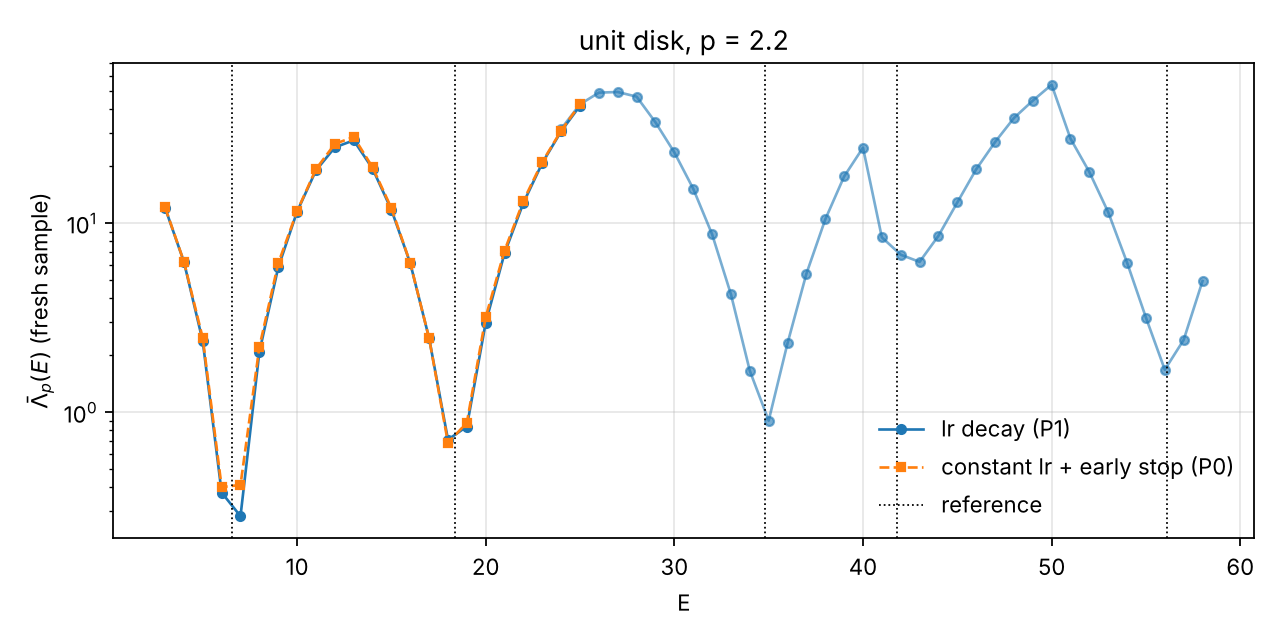
\includegraphics[width=.325\textwidth]{plap_disk_curves.png}
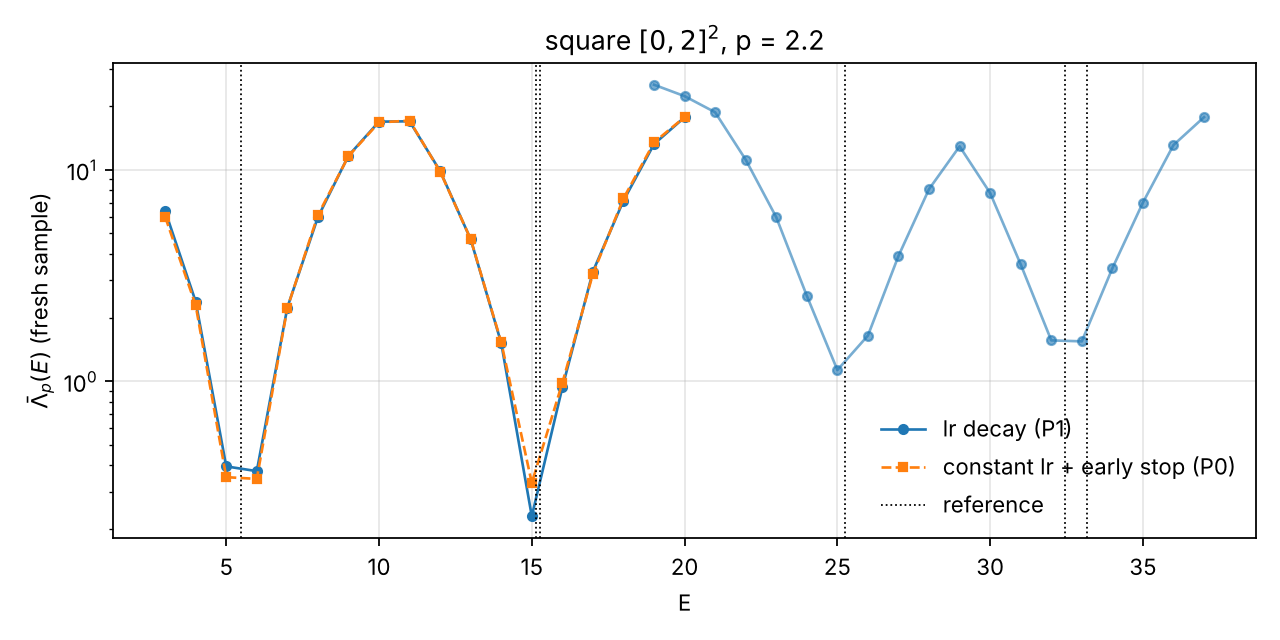
\includegraphics[width=.325\textwidth]{plap_square_curves.png}
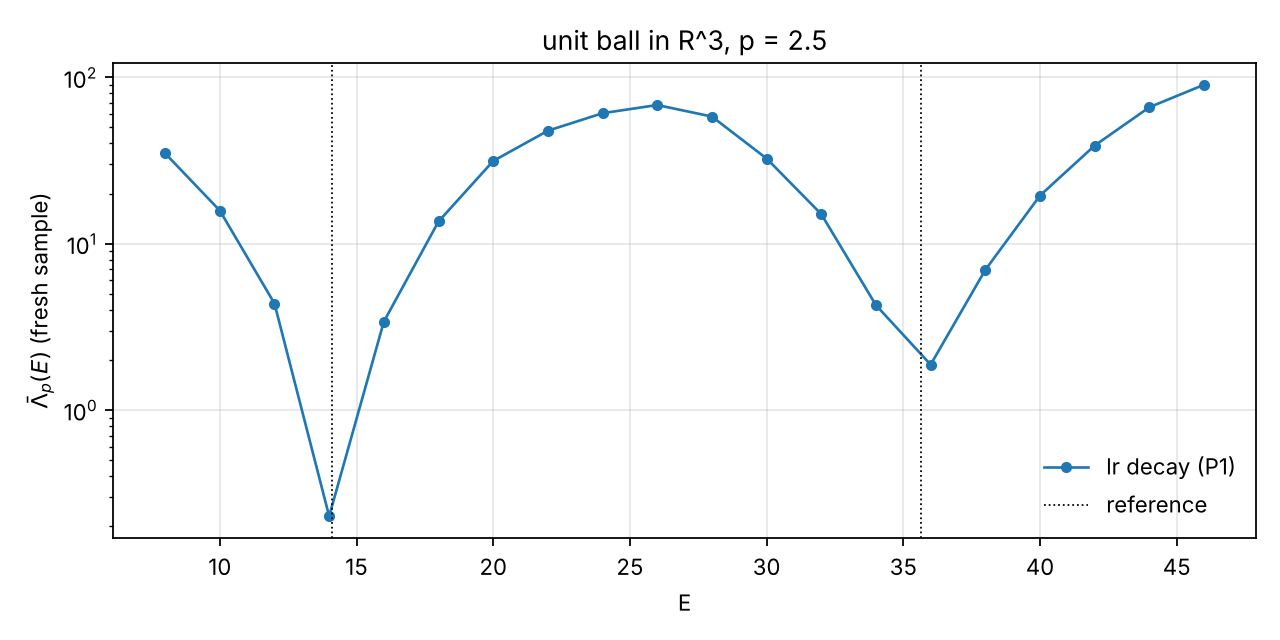
\includegraphics[width=.325\textwidth]{plap_ball_curves.png}
\caption{Loss curves $\bar\Lambda_p(E)$ (fresh sample, logarithmic scale) with the corrected loss: unit disk, $p=2.2$ (left), square $[0,2]^2$, $p=2.2$ (centre), unit ball of $\R^3$, $p=2.5$ (right). Dotted lines: reference eigenvalues. P1: learning-rate decay; P0: constant learning rate with early stopping (protocol of the previous version).}
\label{fig.plap}
\end{figure}

Table~\ref{tab.plap} and Fig.~\ref{fig.plap} show that with the corrected loss the first and second
eigenvalues are reproduced to within $0.1\%$ in the three domains. The \emph{new} result is the
detection of further eigenvalues in the same scan: in the disk, the third to fifth minima match
the eigenvalues with two nodal diameters, one nodal circle and three nodal diameters, and in the
square the third and fourth minima match the $2\times2$ cell mode and the mode with both diagonals
as nodal lines, with errors below $0.1\%$ except for the radial mode with a nodal circle
($+0.41\%$; its gradient vanishes on a whole circle, which gives the largest residual floor). For
the ball of $\R^3$ the shooting value $14.1112$ and the axisymmetric finite element value $35.6315$
are reproduced to $0.08\%$ and $0.01\%$. Two caveats apply. First, close eigenvalues are not
separated: in the square, $15.1429$ (diagonal nodal line) and $15.2808$ (midline nodal line, the
other mode into which the double eigenvalue $5\pi^2/4$ of the Laplacian splits at $p=2.2$) give a
single minimum, as do $32.46$ and $33.17$ (three strips). Second, the reference for $35.63$ is an
eigenvalue of the ball with one nodal plane and an upper bound for the second eigenvalue; that it is
the second eigenvalue is not proved.
\end{revblock}

\subsection{Error sources and convergence}
\begin{revblock}
Table~\ref{tab.plap.conv} varies one setting at a time for the first eigenvalue of the disk,
$p=2.2$. We identify the following error sources.
\begin{enumerate}
\item \emph{Optimization noise.} With the protocol of the previous version (constant learning rate,
early stopping, P0) the loss at a fixed $E$ fluctuates between seeds by $\pm0.1$--$0.2$, while the
curve rises only by $\approx0.27$ at distance $0.5$ from the eigenvalue; the vertex of the curve then
has errors up to $2.3\%$ (three seeds), the size of the errors of the former tables. A decaying
learning rate reduces the fluctuation to $\approx0.01$--$0.02$ and the vertex error to $0.2\%$.
\item \emph{Residual floor near critical points.} After the decay the loss at the eigenvalue is
$\approx0.13$, and $50$--$60\%$ of it comes from the $2\%$ of the sample points with the smallest
$|\nabla u|$, as predicted by Lemma~\ref{lem.critical}. The floor decreases slowly with capacity and
training ($0.150$ for $2\times32$, $0.096$ for $4\times256$; $0.049$ with 5000 epochs), and since it
is not symmetric in $E$ it biases the minimum of the curve by $+0.2$ to $+0.8\%$; this bias is not
removed by a larger network, more points or longer training.
\item \emph{Grid in $E$.} Refining the grid makes the curve estimate \emph{worse}
($+0.18\%$, $+0.78\%$, $+3.7\%$ for $h=0.5,0.25,0.125$), because the differences of the loss between
neighbouring nodes ($\approx c\,h^2$) fall below the fluctuations of the floor. The step should
satisfy $c\,h^2\gg$ (fluctuation), here $h\gtrsim0.5$; a coarse grid followed by the frozen-network
refinement is cheaper and more accurate.
\item \emph{Network capacity and Monte Carlo size} are minor at fixed protocol: $E_{\rm PINN}$ changes
by at most $0.05\%$ from $2\times32$ to $4\times256$ neurons, and by $0.13\%$ for $N=2000$ and $0.00\%$
for $N=20000$.
\end{enumerate}
The refined value $E_{\rm PINN}$ is insensitive to all these settings ($|{\rm error}|\le0.05\%$ for
every configuration with learning-rate decay, $\ge1500$ epochs and $N\ge5000$), because it is computed
from the trained function alone. Hence the loss curve should be used to \emph{detect} the eigenvalues
and the frozen-network quotient to \emph{compute} them.

\begin{table}[tbp]
\centering\small
\color{blue}
\caption{Convergence study for the first eigenvalue of the $p$-Laplacian, $p=2.2$, in the unit disk ($E_1=6.53174$). Each row changes one setting of the baseline ($3\times128$, $N=5000$, 1500 epochs with learning-rate decay, $\mu=200$, $h=0.5$); the loss is sampled at $E=6.0,6.5,7.0$ on $4\cdot10^4$ fresh points. P0: protocol of the previous version.}
\label{tab.plap.conv}
\begin{tabular}{lccccc}
\toprule
setting & $\bar\Lambda_p(6.0)$ & $\bar\Lambda_p(6.5)$ & $\bar\Lambda_p(7.0)$ & $E_{\rm curve}$ (err.\ \%) & $E_{\rm PINN}$ (err.\ \%)\\
\midrule
baseline, seed 0 & 0.394 & 0.131 & 0.316 & 6.543 ($+0.18$) & 6.5320 ($+0.00$)\\
baseline, seed 1 & 0.416 & 0.130 & 0.329 & 6.545 ($+0.20$) & 6.5329 ($+0.02$)\\
baseline, seed 2 & 0.401 & 0.125 & 0.318 & 6.544 ($+0.19$) & 6.5285 ($-0.05$)\\
P0, seed 0 & 0.439 & 0.348 & 0.426 & 6.520 ($-0.17$) & 6.5393 ($+0.12$)\\
P0, seed 1 & 0.427 & 0.204 & 0.338 & 6.562 ($+0.47$) & 6.5453 ($+0.21$)\\
P0, seed 2 & 0.419 & 0.272 & 0.296 & 6.679 ($+2.26$) & 6.5557 ($+0.37$)\\
network $2\times32$ & 0.534 & 0.150 & 0.353 & 6.577 ($+0.69$) & 6.5350 ($+0.05$)\\
network $2\times64$ & 0.467 & 0.137 & 0.348 & 6.555 ($+0.36$) & 6.5343 ($+0.04$)\\
network $4\times256$ & 0.436 & 0.096 & 0.307 & 6.559 ($+0.41$) & 6.5338 ($+0.03$)\\
$N=2000$ & 0.417 & 0.127 & 0.332 & 6.543 ($+0.17$) & 6.5403 ($+0.13$)\\
$N=20000$ & 0.397 & 0.123 & 0.325 & 6.538 ($+0.10$) & 6.5319 ($+0.00$)\\
500 epochs & 0.515 & 0.153 & 0.338 & 6.581 ($+0.76$) & 6.5415 ($+0.15$)\\
5000 epochs & 0.376 & 0.049 & 0.244 & 6.563 ($+0.48$) & 6.5315 ($-0.00$)\\
$\mu=50$ & 0.390 & 0.073 & 0.250 & 6.571 ($+0.60$) & 6.5317 ($-0.00$)\\
$\mu=1000$ & 0.516 & 0.166 & 0.385 & 6.558 ($+0.39$) & 6.5352 ($+0.05$)\\
$h=0.25$ & -- & 0.120 & -- & 6.583 ($+0.78$) & 6.5338 ($+0.03$)\\
$h=0.125$ & -- & 0.116 & -- & 6.773 ($+3.69$) & 6.5337 ($+0.03$)\\
\bottomrule
\end{tabular}
\end{table}
\end{revblock}

\subsection{Range of \texorpdfstring{$p$}{p}}
\begin{revblock}
Table~\ref{tab.plap.p} shows the first eigenvalue of the disk for several $p$. The residual floor of
Lemma~\ref{lem.critical} grows with $p$ (the eigenfunction is only $C^{1,1/(p-1)}$ at its maximum),
and the accuracy degrades from $0.05\%$ ($p=2.2$) to $0.3\%$ ($p=3$) and $1.5\%$ ($p=4$). For $p=1.5$
the method fails: for $p<2$ the strong form $\Delta_pu$ of a smooth network is singular at its
critical points (like $|x-x_0|^{p-2}$), and the Monte Carlo estimator of the loss has infinite variance
for $p\le3/2$ in two dimensions. In its present (strong-form, unregularized) version the method
should therefore be used for $p\ge2$.

\begin{table}[tbp]
\centering\small
\color{blue}
\caption{First eigenvalue of the $p$-Laplacian in the unit disk for several $p$ (baseline settings; reference by radial shooting).}
\label{tab.plap.p}
\begin{tabular}{cccccc}
\toprule
$p$ & $E_1$ (shooting) & $E_{\rm PINN}$ & rel.\ err.\ (\%) & $E_{\rm curve}$ (err.\ \%) & $\bar\Lambda_p^{1/2}$ \\
\midrule
1.5 & 4.0178 & 5.2887 & $+31.6$ & 4.702 ($+17.0$) & 4.92 \\
2.2 & 6.5317 & 6.5320 & $+0.00$ & 6.543 ($+0.18$) & 0.36 \\
3.0 & 9.8315 & 9.8012 & $-0.31$ & 9.885 ($+0.55$) & 0.78 \\
4.0 & 14.6816 & 14.8952 & $+1.45$ & 15.886 ($+8.20$) & 2.50 \\
\bottomrule
\end{tabular}
\end{table}
\end{revblock}


\section{Analysis of the practical method: stability, choice of \texorpdfstring{$\mu$}{mu}, and cost}\label{sec.analysis}

\subsection{Stability of the detection and spurious minima}\label{sec.stability}
\begin{revblock}
The identity \eqref{cota.igual} concerns exact minimizers, whereas the network class $\mathcal N$ of
functions $u=B\,\mathrm{NN}_\theta$ is finite dimensional, training stops after finitely many steps,
and the integrals are sampled. Let $\tilde\Lambda_i$ be the computed (normalized) loss at the node
$E^i=E_*+(i-1)h$. The error splits as
\[
\tilde\Lambda_i-\Lambda(E^i)=
\underbrace{\Lambda(u^i,E^i)-\inf_{\mathcal N}\Lambda(\cdot,E^i)}_{\text{optimization}\ \ge0}
+\underbrace{\inf_{\mathcal N}\Lambda(\cdot,E^i)-\Lambda(E^i)}_{\text{approximation}\ \ge0}
+\underbrace{\tilde\Lambda_i-\Lambda(u^i,E^i)}_{\text{sampling}} ;
\]
since $\mathcal N\subset D(L)$, approximation and optimization errors can only \emph{raise} the loss
curve. We assume only a bound on the total error,
\begin{equation}\label{hyp.delta}
|\tilde\Lambda_i-d(E^i)^2|\le\delta,\qquad i=1,\dots,J,
\end{equation}
and call an interior node $E^m$ a discrete local minimum if
$\tilde\Lambda_m\le\min\{\tilde\Lambda_{m-1},\tilde\Lambda_{m+1}\}$.

\begin{proposition}[Stability of the loss-curve characterization]\label{prop.stability}
Assume \eqref{hyp.delta}, let $\epsilon>0$ be the detection threshold, $\rho=\sqrt{\epsilon+\delta}$
and $\tau=\sqrt{h^2/4+2\delta}$.
\begin{enumerate}
\item[(a)] (No detections away from the spectrum.) If $\tilde\Lambda_i\le\epsilon$, then
$d(E^i)\le\rho$.
\item[(b)] (No missed eigenvalues by thresholding.) Every eigenvalue $E_k\in[E_*,E^*]$ has a node
with $|E^i-E_k|\le h/2$ and $\tilde\Lambda_i\le h^2/4+\delta$; hence all of them are detected if
$\epsilon\ge h^2/4+\delta$.
\item[(c)] (Local minima are close to the spectrum.) Every discrete local minimum satisfies
$d(E^m)\le\max\{h,\ h/2+\delta/h\}$, irrespective of its value.
\item[(d)] (Isolated eigenvalues produce local minima.) If
$[E_k-\tau-h,E_k+\tau+h]\subset[E_*,E^*]$ and $\dist(E_k,\sigma\setminus\{E_k\})>2\tau+h$, there is a
discrete local minimum $E^m$ with $|E^m-E_k|\le\tau$.
\end{enumerate}
\end{proposition}
The proof is given in Appendix~\ref{app.proofs}.

\begin{remark}[Interpretation]\label{rem.stability}
(1) Imperfect training cannot create detections far from the spectrum: every node below the
threshold, and every discrete local minimum, lies within an explicit distance of a true
eigenvalue. What it can do is produce several minima around the same eigenvalue, or raise the curve
above the threshold so that an eigenvalue is missed. Refining the grid below $h\simeq\sqrt{2\delta}$
does not improve the localization (the bound in (c) is minimal there). (2) The loss curve only sees
the set $\sigma$: a multiple eigenvalue produces a single minimum and the network converges to some
element of the eigenspace. Multiplicities would have to be recovered separately, e.g.\ by training
at the detected value from several initializations and computing the rank of the Gram matrix of
the resulting functions; we have not implemented this. (3) Two eigenvalues are separated by a bump of
height $(E_{k+1}-E_k)^2/4$; if $E_{k+1}-E_k\le2\sqrt{2\delta}$ the bump is below the error level and
the number of eigenvalues in such a cluster cannot be determined from the curve: the method returns
the cluster as a single approximate eigenvalue (Section~\ref{sec.fem}). (4) Proposition
\ref{prop.stability} is conditional on \eqref{hyp.delta}; we do not prove a bound on $\delta$ in terms
of the network size, the number of epochs and of sampling points. The approximation error tends to
zero as the width grows (networks with smooth non-polynomial activation are dense in
$C^2(\overline\Omega)$ \cite{Hornik1991,Pinkus1999}; rates for $\tanh$ networks are given in
\cite{DeRyck-Lanthaler-Mishra}), but no convergence guarantee for the optimizer is available, and the
spectral bias of gradient-based training \cite{Rahaman-etal} suggests that $\delta$ grows with $E$,
in agreement with the residuals in our tables. The error can, however, always be \emph{measured} a
posteriori (Section~\ref{sec.certificate}).
\end{remark}

\emph{Experiments.} (i) Seeds. We scanned the window $[15,55]$ of the unit square (step 5,
$\mu=450$, settings of Section~\ref{sec.implementation}) with three seeds. All
three runs gave local minima at $E=20$ and $E=50$ only, i.e.\ no spurious minimum, and refined values
$19.7394$, $19.7397$, $19.7450$ for $2\pi^2$ and $49.3486$, $49.3485$, $49.3474$ for $5\pi^2$. In all
cases the Weinstein bound $|\hat E-E_k|\le r$ held with two to three orders of magnitude to spare
($r=0.16$--$0.68$) and the Kato--Temple bound $r^2/\gamma$ held as well (it exceeded the actual error by
a factor $5$--$25$). (ii) Collapse. Spurious zeros of the \emph{recorded} curve were observed, but
only in one form: the collapse to the trivial state $u\equiv0$. In the scan of Table~\ref{table.1}
the network was re-initialized at $E=99.7$, collapsed to $u\equiv0$ and stayed there up to $E=105$
(Fig.~\ref{fig.collapse}). The recorded residual term dropped to $\approx10^{-5}$, the lowest value of
the whole curve, which any threshold would accept; but the mean of $u^2$ was $\approx10^{-8}$ and the
certificate radius $r$ was $30$--$42$. Collapsed nodes are therefore detected by $\overline{u^2}\approx0$
and a large $r$, and are invisible in the residual term alone. The same happens when $\mu$ is too
small (Section~\ref{sec.mu}). We therefore record, at each node, the normalized loss
$\Lambda(u,E)=r^2$ and the mass $\overline{u^2}$, and discard nodes with $\overline{u^2}<\frac12$.


\begin{figure}[tbp]
\centering
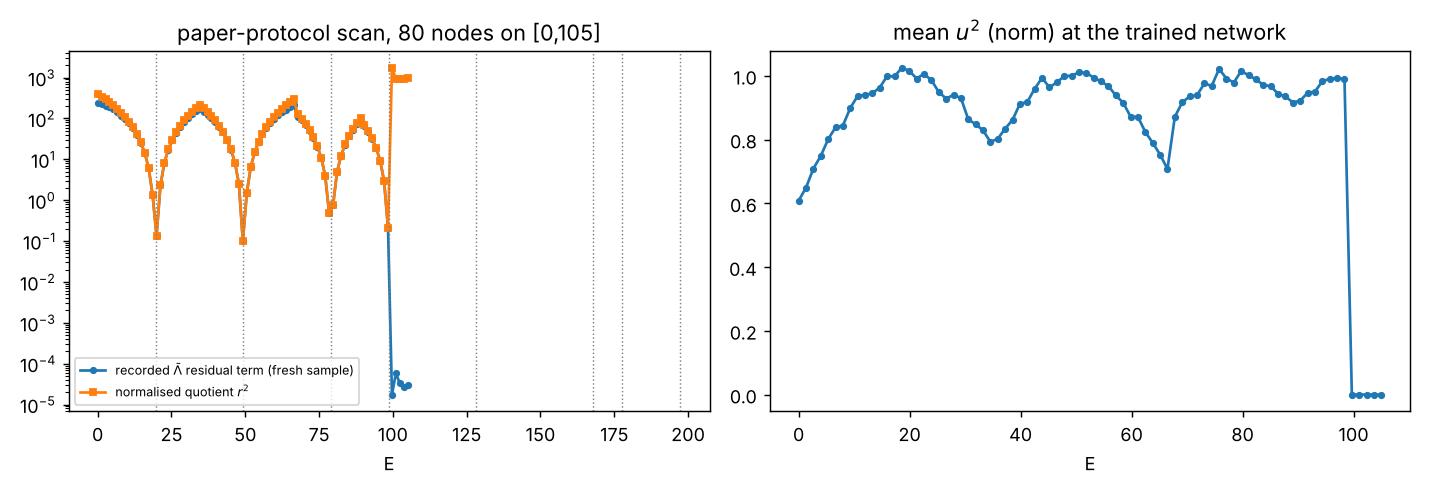
\includegraphics[width=.75\textwidth]{paper_sweep_curve.png}
\caption{The scan of Table~\ref{table.1} (80 nodes on $[0,105]$, $\mu=500$). Left: recorded residual term and normalized loss $r^2$ (dotted lines: eigenvalues). Right: mean of $u^2$. After the re-initialization at $E=99.7$ the network collapses to $u\equiv0$: the recorded residual drops to $10^{-5}$ while $r^2$ jumps to $\approx10^3$.}
\label{fig.collapse}
\end{figure}
\end{revblock}

\subsection{Choice of the penalty parameter}\label{sec.mu}
\begin{revblock}
In the previous version $\mu$ was chosen with the heuristic $\mu\propto E^2$. Proposition
\ref{prop.penalized} gives a precise rule. Let $[E_*,E^*]$ be the window and
\[
D=\max_{E\in[E_*,E^*]}d(E),
\]
i.e.\ half of the largest gap between consecutive eigenvalues meeting the window, or the distance from
an endpoint of the window to the spectrum if this is larger. Let $R_\mu(E)$ be the residual term of
\eqref{lossmu} at the minimizer, which is the quantity recorded during the scan.

\begin{corollary}\label{cor.mu}
(i) For every $\mu>0$ the zeros of $\bar\Lambda(E)$ are exactly the eigenvalues, and
$0\le d^2-\bar\Lambda(E)\le d^4/(4\mu)$ when $d^2\le2\mu$. (ii) If $\mu\ge D^2$, then
$\|u_E\|_2^2\ge\frac12$ and $R_\mu(E)=d^2(1-d^2/(2\mu))$ is an increasing function of $d=d(E)$ on the
window: its zeros and local minima are exactly the eigenvalues. (iii) If $\frac12D^2\le\mu<D^2$,
$R_\mu$ has spurious local minima where $d$ has a local maximum larger than $\sqrt\mu$. (iv) If
$\mu<\frac12D^2$, the minimizer is $u_E=0$ wherever $d(E)^2\ge2\mu$, and the recorded curve has
spurious zeros there.
\end{corollary}
This follows directly from Proposition~\ref{prop.penalized}, since $R_\mu=\psi(d^2)$ with
$\psi(t)=t(1-t/(2\mu))_+$, which increases on $[0,\mu]$, decreases on $[\mu,2\mu]$ and vanishes for
$t\ge2\mu$. The location of the minima does not depend on $\mu$, and the normalized quotient
$\Lambda(u_E,E)=d(E)^2$ is independent of $\mu$.

\emph{Guideline.} (1) Along a warm-started scan it suffices to take $\mu\ge D^2$; we recommend
$\mu\approx2D^2$. $D$ can be estimated from Weyl's law or from a coarse preliminary scan. Since the
gaps do not grow with $E$ in dimension $d\ge2$, $\mu$ need not grow with $E$. (2) When the network is
trained \emph{from scratch} at a level $E$ (cold start, or periodic re-initialization), the residual
of the initial network is of order $E^2$ and the amplitude decreases towards $u=0$ unless
$\mu\gtrsim\frac12E^2$; this is the correct form of the former heuristic, and it only concerns cold
starts. (3) A very large $\mu$ is harmful: the sampled penalty adds a noise floor
$\mu\operatorname{Var}(u^2)/N$ to the loss and makes the problem stiff. In our examples $\mu$ ranged from
$100$ to $15000$; in the triangle, for instance, the window $[0,180]$ starts far below
$E_1=5\pi^2$, so $D=5\pi^2$ and $D^2\approx2435$, while $\mu=15000$ lies between $D^2$ and the
cold-start scale $E^2/2$.

\emph{Sensitivity study.} We scanned the window $[40,60]$ of the unit square, which contains only
$5\pi^2=49.348$ (double) and has $D=10.65$, $D^2=113.5$, with step 2 and warm start, two seeds and
nine values of $\mu$ from $1$ to $10^4$. To keep the cost manageable we used a reduced network
($3\times64$, 3000 points, at most 2000 epochs); at $\mu=1000$ it gave the same normalized loss values
and Rayleigh quotients as the full network ($3\times128$, 5000 points) to within the training noise.
Table~\ref{table.mu} and Fig.~\ref{fig.mu} show the results.

\begin{table}[tbp]
\centering\small
\color{blue}
\caption{Sensitivity to $\mu$ (unit square, window $[40,60]$, $D^2=113.5$, step 2, two seeds, reduced network). Collapsed nodes: nodes with $\overline{u^2}<0.1$, observed (max over seeds) / predicted by Proposition~\ref{prop.penalized}. Minima: of the recorded residual term. $\hat E$: Rayleigh quotient at the minimum near $5\pi^2$, seed 0.}
\label{table.mu}
\begin{tabular}{rrcccc}
\toprule
$\mu$ & $\mu/D^2$ & collapsed nodes (obs./pred.) & minima of recorded curve & $\hat E$ & rel.\ err.\\
\midrule
1 & 0.009 & 11/10 & spurious only & -- & --\\
10 & 0.09 & 11/7 & spurious only & -- & --\\
30 & 0.26 & 5/3 & 42 (spurious), 50 & 49.3465 & $3\times10^{-5}$\\
60 & 0.53 & 2/1 & 50 & 49.3474 & $1\times10^{-5}$\\
100 & 0.88 & 0/0 & 50 & 49.3476 & $9\times10^{-6}$\\
113 & 1.0 & 0/0 & 50 & 49.3479 & $2\times10^{-6}$\\
300 & 2.6 & 0/0 & 50 & 49.3478 & $4\times10^{-6}$\\
1000 & 8.8 & 0/0 & 50 & 49.3485 & $1\times10^{-5}$\\
10000 & 88 & 0/0 & 50 & 49.3580 & $2\times10^{-4}$\\
\bottomrule
\end{tabular}
\end{table}

\begin{figure}[tbp]
\centering
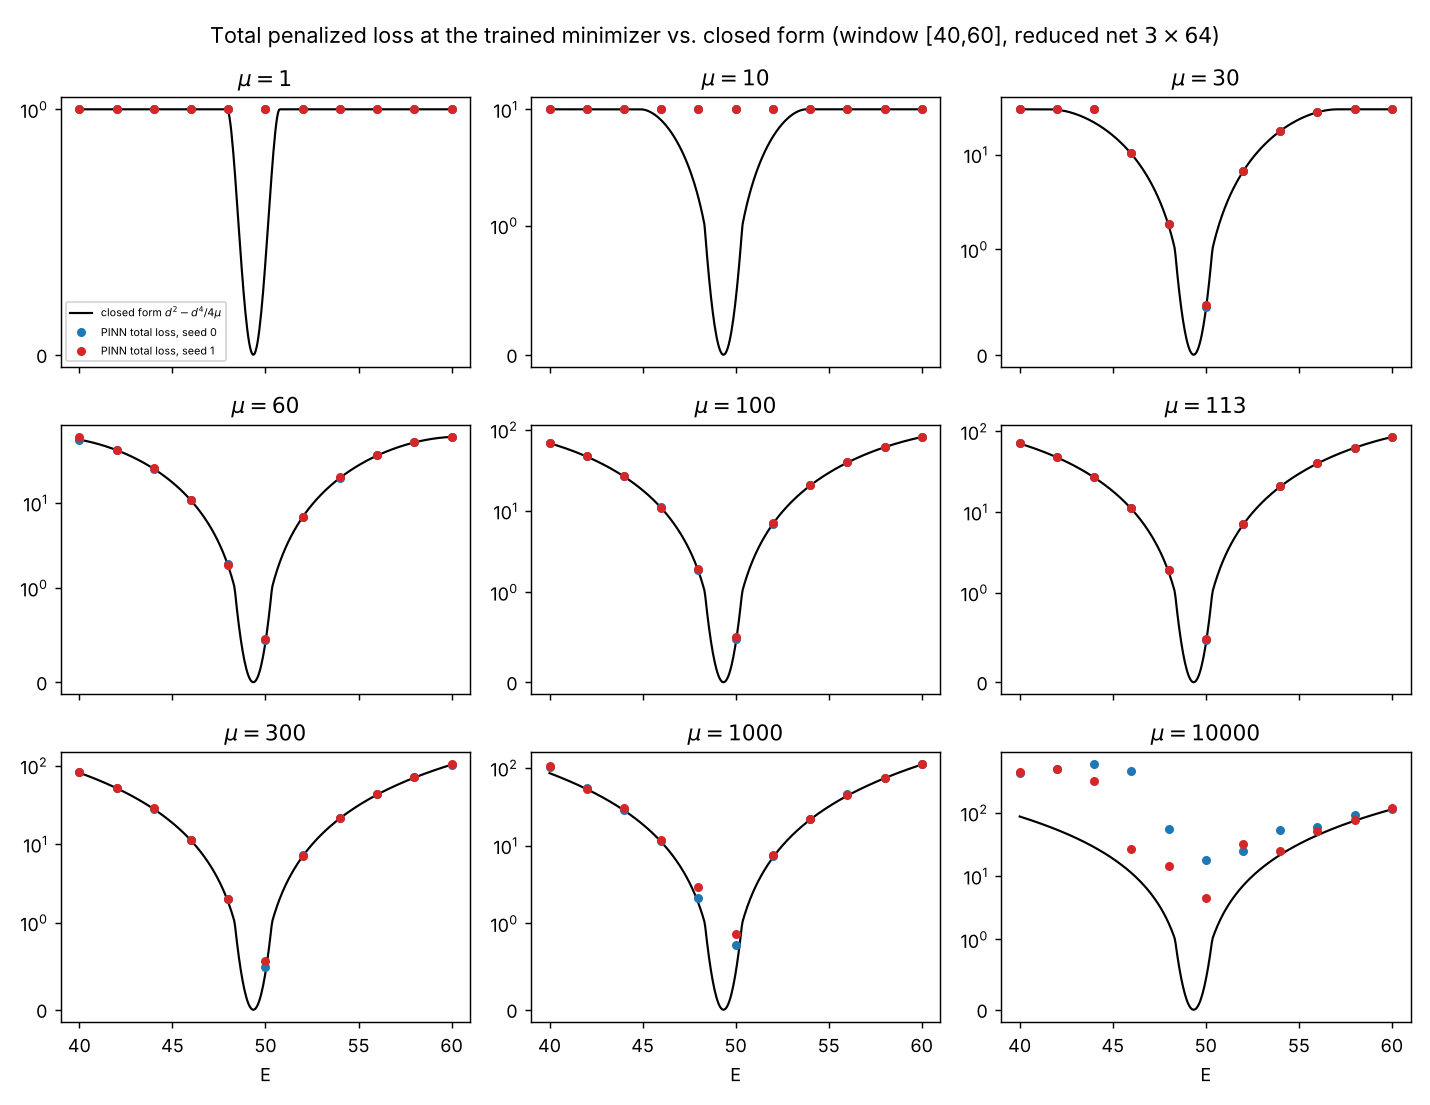
\includegraphics[width=.62\textwidth]{mu_loss_curves.png}
\caption{Total penalized loss at the trained networks (dots, two seeds) and the closed form $d^2-d^4/(4\mu)$ of Proposition~\ref{prop.penalized} (solid line), window $[40,60]$ of the unit square, for the nine values of $\mu$ of Table~\ref{table.mu}.}
\label{fig.mu}
\end{figure}

The computed eigenvalue is flat in $\mu$ over $[60,10^4]$ (relative error below $2\times10^{-4}$), and
the curves follow the closed form for $60\le\mu\le1000$ (the mean of $u^2$ follows the prediction
$1-d^2/(2\mu)$ with an RMS deviation $\approx0.01$ for $\mu\ge100$). The thresholds are confirmed: for
$\mu<D^2/2=57$ the network collapses at the far nodes (for $\mu=1,10$ at all nodes, more than predicted,
because a warm-started $u\approx0$ is not left), and at $\mu=30$ the recorded residual has a spurious
zero at $E=42$, whereas the normalized loss $r^2$ has a single minimum at $E=50$ for all $\mu\ge30$.
For $\mu=10^4$ the minimum is still at the right place but the curve is distorted (stiff penalty, not
converged in 2000 epochs). The cold-start condition was also confirmed: started from scratch on
$[95,102]$, the scan collapsed at every node with $\mu=450$, while $\mu=5000>(102)^2/2$ gave
$10\pi^2$ with relative error $2.1\times10^{-5}$.
\end{revblock}

\subsection{Computational cost}\label{sec.cost}
\begin{revblock}
\emph{Cost model.} Let $W$ be the number of network parameters, $N$ the number of sampling points and
$d$ the dimension. The loss \eqref{lossmu} needs $\Delta u_\theta$, i.e.\ one backward pass for
$\nabla u_\theta$ and $d$ further passes for the diagonal of the Hessian, so one epoch costs
$c_{\rm ep}=\kappa(d+2)NW$, linear in $d$. If $n_i$ epochs are used at node $E^i$, the scan of a
window with $J$ nodes costs
\begin{equation}\label{cost.scan}
C_{\rm scan}=c_{\rm ep}\sum_{i=1}^Jn_i\le\kappa(d+2)NWJn_{\max}.
\end{equation}
By Proposition~\ref{prop.stability} the grid only needs to separate the eigenvalues, $h\lesssim
\gamma_{\min}/2$, since the accuracy comes from the Rayleigh quotient and not from $h$; hence
$J\approx2(E^*-E_*)/\gamma_{\min}$. With warm start most nodes need few epochs (in the scan of
Table~\ref{table.1}, $302$--$3060$ epochs per node, median $\approx500$, against a maximum of $5000$). The
trainings at different nodes, or in different sub-windows each with its own warm start, are
independent, so the wall-clock time can be divided by the number of processors. A Rayleigh-quotient
PINN with deflation \cite{Rowan-Evans-Maute-Dootsan,Holliday-Lindner-Ditto,E-Yu} computes the
$k$-th eigenpair by minimizing $R(u)$ plus penalties for the overlap with the $k-1$ previous networks;
an epoch needs only first derivatives (cost $\kappa'NW$) plus the evaluation of the previous networks,
so the first $K$ eigenpairs cost $\approx\bar n\,NW(\kappa'K+\frac{c_0}2K^2)$, sequentially, and errors
in the computed eigenfunctions bias all subsequent eigenvalues downwards (Courant--Fischer).

\emph{Measurements.} We compared both approaches on the unit square with the same network, boundary
factor and sample size, on one CPU thread (Table~\ref{table.cost}). The deflation baseline
minimizes $R(u)$ plus $\beta\sum_{j<k}\langle u,u_j\rangle^2/(\|u\|^2\|u_j\|^2)$ with $\beta=200$; the
eigenvalue is its Rayleigh quotient.

\begin{table}[tbp]
\centering\small
\color{blue}
\caption{Cost on the unit square (one CPU thread, $3\times128$ network, 5000 points per epoch, shared machine: times indicative). The six lowest eigenvalues counted with multiplicity are $2\pi^2$, $5\pi^2$ (double), $8\pi^2$, $10\pi^2$ (double).}
\label{table.cost}
\begin{tabular}{lrll}
\toprule
method & wall time (s) & eigenvalues obtained & max.\ rel.\ error\\
\midrule
Rayleigh + deflation, $K=6$, early stopping & 241--317 & 6 (with multiplicity) & $3\times10^{-2}$\\
Rayleigh + deflation, $K=6$, no early stopping & 817 & 6 (with multiplicity) & $1.3\times10^{-3}$\\
Rayleigh + deflation, first 5 (to reach $10\pi^2$) & 253 / 647 & 5 & $3\times10^{-2}$ / $1.3\times10^{-3}$\\
Scan $[15,105]$, $h=5$, 19 nodes, $\mu=450$ & 2077 (+99) & 4 distinct & $2.4\times10^{-5}$\\
Scan $[0,105]$, 80 nodes (Table~\ref{table.1}) & 6534 (+413) & 4 distinct & $3.5\times10^{-5}$\\
Scan $[95,102]$ only, 5 nodes, cold start, $\mu=5000$ & 950 (+24) & $10\pi^2$ & $2.1\times10^{-5}$\\
\bottomrule
\end{tabular}
\end{table}

The times in parentheses are those of the refinement. The comparison is clear: for the lowest
eigenvalues of a two-dimensional problem the Rayleigh-quotient PINN with deflation is \emph{cheaper}
in raw wall time (by a factor $\approx7$--$29$ for all six eigenvalues, and by a factor $1.5$--$4$ even
when the scan targets $10\pi^2$ directly), and it \emph{resolves multiplicities}, which the scan does
not. The scan gave more accurate values in these runs, but this is mainly a matter of training
length: the deflation errors drop from $3\times10^{-2}$ to $1.3\times10^{-3}$ without early stopping,
and the deflated eigenfunctions accumulate errors (the second eigenvalue was the least accurate). The
advantages of the scan lie elsewhere: (i) the nodes and windows are independent and can be computed in
parallel (not exploited in the timings above), whereas deflation is sequential; (ii) each detected
eigenvalue carries its own a posteriori enclosure (Weinstein, Kato--Temple), computed from the
corresponding network alone and independent of the accuracy of other eigenpairs; (iii) a high
eigenvalue can be targeted without computing the lower ones, so its cost depends on the window and
not on the index (for deflation the number of lower eigenvalues grows like $E^{d/2}$ by Weyl's law);
(iv) the scan applies verbatim to nonlinear problems such as the $p$-Laplacian, where no orthogonality
is available. Its limitations are equally clear: the cost of a full scan is (number of nodes)
$\times$ (cost of one training), the second derivatives make each epoch more expensive, and
multiplicities and close clusters are not resolved (Remark~\ref{rem.stability}).
\end{revblock}

\section{Conclusions}\label{sec.conclusions}

The method proposed in this work provides a flexible framework for computing eigenvalues and eigenfunctions of differential operators using neural networks. \rev{The detection step does not rely on the Rayleigh quotient or on orthogonality conditions between eigenfunctions; in the linear case the Rayleigh quotient of the detected network is then used to refine the value and to certify it.} As a result, it is well-suited for computing \rev{eigenvalues in a prescribed window} and for addressing nonlinear problems where such structures are no longer available.

\begin{revblock}
For self-adjoint problems the loss curve equals the squared distance to the spectrum; the penalized
loss used in practice has an explicit loss curve and no spurious local minima, which yields the rule
$\mu\ge D^2$ (warm start) and $\mu\gtrsim E^2/2$ (cold start), confirmed by a sensitivity study. The
detection is stable under training and sampling errors, the only spurious zeros observed came from
the collapse $u\equiv0$, which is detected by the mass and the certificate, and each eigenvalue comes
with an a posteriori enclosure. The method was validated against exact values and independent finite
element computations in dimensions two to four (errors below $0.1\%$ for the potentials). For the
$p$-Laplacian, after correcting the loss of the previous version, the first and second eigenvalues
are reproduced to within $0.1\%$, further eigenvalues are detected in the same scan, and the dominant
error sources (optimization noise and the residual floor at critical points) have been identified; the
method works for $p\ge2$.

\emph{Limitations.} The scan does not resolve multiplicities or clusters of eigenvalues closer than
the error level; eigenvalues can be missed when the warm-started network stays on a neighbouring branch
(annulus, harmonic potential with $\omega=10$); for the lowest eigenvalues of linear problems a
Rayleigh-quotient PINN with deflation is cheaper, and finite elements are much cheaper and more
accurate in the dimensions considered here; no bound on the training error is proved; and for the
$p$-Laplacian there is no a posteriori certificate and the method in its present form fails for
$p<2$.
\end{revblock}

\section*{Declarations}

\subsection*{Code availability}
\rev{The Python code used in this work, including the scripts and raw results of all the experiments
of this version, is openly accessible at}
\begin{center}
\rev{\url{https://github.com/jfbonder/PINN-eigenvalues-v2}}
\end{center}

\subsection*{\rev{Data availability}}
\rev{No external data were used; all data are generated by the code above.}

\subsection*{\rev{Conflict of interest}}
\rev{The authors declare that they have no conflict of interest.}
% TODO (authors): confirm the conflict-of-interest statement and add any further declaration
% required by the journal template (e.g. author contributions, use of AI tools).

\subsection*{Funding}
This work was partially supported by ANPCyT under grant PICT 2019-3837 and by CONICET under grant PIP 11220150100032CO.

\subsection*{Acknowledgements}
JFB thanks Pablo Groisman for encouraging him to teach a course on the Mathematical Foundations of Deep Learning in the fall semester of 2025, which inspired \rev{this work}.


\appendix

\section{The minimization problem}

In this appendix, we show that the minimization problem leading to the loss curve $\Lambda(E)$ defined in \eqref{loss-curve} admits a solution. In order to keep things simple, we consider the case in which $V(x)$ is \rev{the hard-wall} potential \eqref{conf.V} with $\Omega\subset \R^{\rev{d}}$ bounded. \rev{(Given \eqref{cota.igual}, the existence also follows from the spectral decomposition, the minimizers being the eigenfunctions of the eigenvalue(s) closest to $E$; the proof below does not use the spectral theorem.)}

To this end, we must specify the function space over which the infimum is taken. The natural choice is the Sobolev space $H^2(\Omega) \cap H^1_0(\Omega)$. The main result of this section reads as follows:

\begin{theorem}\label{teo.min}
Let $V(x)$ be as in \eqref{conf.V} with $\Omega\subset \R^{\rev{d}}$ bounded \rev{and either convex or of class $C^{1,1}$}. Given \rev{$E\in\R$}, there exists $u_E\in H^2(\Omega)\cap H^1_0(\Omega)$ such that
$$
\Lambda(E) = \Lambda(u_E, E) = \inf_{u\in H^2(\Omega)\cap H^1_0(\Omega)\rev{\setminus\{0\}}}\Lambda(u, E),
$$
where $\Lambda(u, E)$ is given in \eqref{Lambda}.
\end{theorem}

\begin{proof}
The result follows from the \emph{direct method in the Calculus of Variations}. Fix \rev{$E\in\R$}, and consider a minimizing sequence $\{u_j\}_{j \in \N} \subset H^2(\Omega) \cap H^1_0(\Omega)$ such that $\|u_j\|_2 = 1$ and
$$
\Lambda(E) = \lim_{j \to \infty} \Lambda(u_j, E).
$$
In particular, the sequence $\Lambda(u_j, E)$ is bounded and nonnegative:
\begin{equation}\label{cota.Lambda}
0 \le \Lambda(u_j, E) \le C,
\end{equation}
for some constant $C > 0$. Now observe that
\begin{align*}
\Lambda(u_j, E) &= \int_\Omega (\Delta u_j + Eu_j)^2\, dx = \int_\Omega (\Delta u_j)^2\, dx + 2E\int_\Omega u_j \Delta u_j \, dx+ E^2.
\end{align*}
\rev{If $E=0$ there is nothing to do. Otherwise, using} the inequality $ab\le \theta a^2 + \frac{b^2}{4\theta}$ for any $a, b\rev{\ge}0$ and $\theta >0$ we estimate:
$$
\int_\Omega |u_j| |\Delta u_j|\, dx \le \theta \int_\Omega (\Delta u_j)^2\, dx + \frac{1}{4\theta}\int_\Omega u_j^2\, dx.
$$
Taking \rev{$\theta=1/(4|E|)$}, we obtain \rev{$2|E|\int_\Omega|u_j||\Delta u_j|\,dx\le\frac12\int_\Omega(\Delta u_j)^2\,dx+2E^2$, and therefore}
\begin{equation}\label{cota.Lambda2}
\Lambda(u_j, E)\ge \frac12 \int_\Omega (\Delta u_j)^2\, dx \rev{-E^2}.
\end{equation}
Combining \eqref{cota.Lambda}, \eqref{cota.Lambda2} \rev{we get $\|\Delta u_j\|_2^2\le2(C+E^2)$. Since $\Omega$ is convex or of class $C^{1,1}$, $\|u\|_{H^2(\Omega)}\le C_\Omega\|\Delta u\|_2$ for $u\in H^2(\Omega)\cap H^1_0(\Omega)$, so} the sequence $\{u_j\}_{j\in\N}$ is bounded in $H^2(\Omega)\cap H^1_0(\Omega)$.

Therefore, up to a subsequence, we have $u_j \rightharpoonup u_E$ weakly in $H^2(\Omega) \cap H^1_0(\Omega)$ for some $u_E$ in that space.

Since the functional
$$
u \mapsto \int_\Omega (\Delta u + E u)^2\, dx
$$
is convex in $u$, it is weakly lower semicontinuous. Thus,
$$
\int_\Omega (\Delta u_E + E u_E)^2\, dx \le \liminf_{j \to \infty} \int_\Omega (\Delta u_j + E u_j)^2\, dx.
$$
Moreover, the \rev{embedding} $H^2(\Omega)\cap H^1_0(\Omega)\hookrightarrow L^2(\Omega)$ is compact, so
$$
\int_\Omega u_E^2\, dx = \lim_{j\to\infty} \int_\Omega u_j^2\, dx = 1.
$$
Hence, $u_E$ is admissible and attains the minimum.
\end{proof}

\section{Proofs of the new results}\label{app.proofs}
\begin{revblock}
Throughout, $L$, $u_k$, $E_k$, $d(E)$ are as in Section~\ref{sec.approach} and $\|\cdot\|=\|\cdot\|_2$.

\begin{proof}[Proof of Proposition~\ref{prop.penalized}]
Write $u=\sum_kc_ku_k$, $s=\|u\|^2$. Then $\|(L-E)u\|^2=\sum_k(E_k-E)^2c_k^2\ge d^2s$, with equality
iff $u\in N_E$, the span of the eigenfunctions with $|E_k-E|=d$. Hence
$\bar\Lambda(u,E)\ge g(s):=d^2s+\mu(s-1)^2$, with equality iff $u\in N_E$. If $d^2<2\mu$, $g$ attains its
minimum on $[0,\infty)$ only at $s_*=1-d^2/(2\mu)$, with $g(s_*)=d^2-d^4/(4\mu)$; if $d^2\ge2\mu$, $g$ is
increasing and its minimum is $g(0)=\mu$. This gives the formula and the minimizers; the residual term
at the minimizer is $d^2s_*$. For the critical points, the derivative of $\bar\Lambda(\cdot,E)$ at $u$ in
the direction $u_k$ is $2[(E_k-E)^2-2\mu(1-s)]c_k$, so $u\ne0$ is critical iff all $k$ with
$c_k\ne0$ share the same $\lambda=(E_k-E)^2$ and $s=1-\lambda/(2\mu)$ (thus $\lambda<2\mu$). If
$\lambda>d^2$ and $u_j$ is an eigenfunction with $|E_j-E|=d$, then $c_j=0$ and
$\bar\Lambda(u+tu_j,E)=\bar\Lambda(u,E)+t^2(d^2-\lambda)+\mu t^4$, which is smaller for small $t\ne0$; so
$u$ is a saddle. Likewise $\bar\Lambda(tu_j,E)=\mu+t^2(d^2-2\mu)+\mu t^4$, so $u=0$ is not a local
minimizer if $d^2<2\mu$. The critical points with $\lambda=d^2$ are the global minimizers.
\end{proof}

\begin{proof}[Proof of Proposition~\ref{prop.rayleigh}]
Assume $\|u\|=1$, $u=\sum_jc_ju_j$, $\rho=\rho(u)$, $\eta=\eta(u)$. (a) follows from
$\|(L-E)u\|^2=\|(L-\rho)u\|^2+(\rho-E)^2$, since $\langle(L-\rho)u,u\rangle=0$. (b) $\|(L-E)u\|^2=
\sum_j(E_j-E)^2c_j^2\ge d(E)^2$. (c) Let $\beta=\rho+\gamma$. Since $\sigma\cap(E_k,\beta)=\emptyset$,
$(E_j-E_k)(E_j-\beta)\ge0$ for all $j$; expanding around $\rho$ and using $\sum c_j^2=1$,
$\sum c_j^2(E_j-\rho)=0$, $\sum c_j^2(E_j-\rho)^2=\eta^2$ gives $0\le\eta^2+(\rho-E_k)(\rho-\beta)$, i.e.\
$\rho-E_k\le\eta^2/\gamma$. The lower bound follows in the same way with $\alpha=\rho-\gamma$.
\end{proof}

\begin{proof}[Proof of Proposition~\ref{prop.stability}]
Write $d_i=d(E^i)$. (a) $d_i^2\le\tilde\Lambda_i+\delta\le\epsilon+\delta$. (b) Some node satisfies
$|E^i-E_k|\le h/2$, and then $\tilde\Lambda_i\le d_i^2+\delta\le h^2/4+\delta$. (c) Let $E_k$ be the
eigenvalue with $|E^m-E_k|=d_m$ and assume $d_m\ge h$. The neighbour $E^{m'}$ on the side of $E_k$ has
$d_{m'}\le d_m-h$, so $d_m^2-\delta\le\tilde\Lambda_m\le\tilde\Lambda_{m'}\le(d_m-h)^2+\delta$, i.e.\
$2hd_m\le h^2+2\delta$. (d) Let $I=[E_k-\tau-h,E_k+\tau+h]$ and let $E^m$ minimize $\tilde\Lambda$ over
the nodes in $I$. By (b), $\tilde\Lambda_m\le h^2/4+\delta$, hence $d_m\le\tau$. If the eigenvalue closest
to $E^m$ were $E_j\ne E_k$, then $|E^m-E_k|\ge\gamma_k-\tau>\tau+h$, contradicting $E^m\in I$; hence
$|E^m-E_k|\le\tau$, both neighbours of $E^m$ lie in $I$, and $E^m$ is a discrete local minimum.
\end{proof}

\begin{proof}[Proof of Proposition~\ref{prop.plap}]
(a) Since $\Delta_pu_k=-E_k|u_k|^{p-2}u_k$, the residual is $(E-E_k)|u_k|^{p-2}u_k$ and the penalty
vanishes. (b) If $E\in\sigma_p$, $\Lambda_p(E)=0$ by (a). Conversely, by the homogeneity
$\Delta_p(tu)=|t|^{p-2}t\Delta_pu$, every $u\ne0$ can be written as $tw$ with $\|w\|_p=1$, and
$\bar\Lambda_p(tw,E)=t^{2(p-1)}Q(w)+\mu(t^p-1)^2$ with $Q(w)=\int(\Delta_pw+E|w|^{p-2}w)^2$; hence
$\Lambda_p(E)=0$ forces $\inf_{\|w\|_p=1}Q(w)=0$. Take $w_n$ with $\|w_n\|_p=1$ and
$f_n:=-\Delta_pw_n-E|w_n|^{p-2}w_n\to0$ in $L^2$. Testing with $w_n$ and using
$\|w\|_2\le C_S\|\nabla w\|_p$ (here $p\ge2d/(d+2)$ is used),
$\|\nabla w_n\|_p^p\le E+C_S\|f_n\|_2\|\nabla w_n\|_p$, so $w_n$ is bounded in $W^{1,p}_0$. Up to a
subsequence $w_n\rightharpoonup w$ in $W^{1,p}_0$ and $w_n\to w$ in $L^p$, so $\|w\|_p=1$ and
$|w_n|^{p-2}w_n\to|w|^{p-2}w$ in $L^{p'}\subset W^{-1,p'}$; also $f_n\to0$ in $W^{-1,p'}$. Thus
$-\Delta_pw_n\to E|w|^{p-2}w$ in $W^{-1,p'}$, and by continuity of $(-\Delta_p)^{-1}\colon
W^{-1,p'}\to W^{1,p}_0$, $w_n\to w$ strongly, with $-\Delta_pw=E|w|^{p-2}w$, $w\ne0$.
\end{proof}
\end{revblock}

\begin{thebibliography}{99}

\bibitem{Lu-Meng-Mao}
L.~Lu, X.~Meng, Z.~Mao, and G.~E. Karniadakis,
DeepXDE: a deep learning library for solving differential equations,
SIAM Rev. \textbf{63}, 208 (2021).

\bibitem{Rackauckas}
C.~Rackauckas, Y.~Ma, J.~Martensen, C.~Warner, K.~Zubov, R.~Supekar, D.~Skinner, A.~Ramadhan, and A.~Edelman,
Universal differential equations for scientific machine learning (2021),
\href{https://arxiv.org/abs/2001.04385}{arXiv:2001.04385 [cs.LG]}.

\bibitem{Rackauckas-Innes-Ma-Bettencourt-etal}
C.~Rackauckas, M.~Innes, Y.~Ma, J.~Bettencourt, L.~White, and V.~Dixit,
DiffEqFlux.jl -- a Julia library for neural differential equations (2019),
\href{https://arxiv.org/abs/1902.02376}{arXiv:1902.02376 [cs.LG]}.

\bibitem{Blechschmidt-Ernst}
J.~Blechschmidt and O.~G. Ernst,
Three ways to solve partial differential equations with neural networks---a review,
GAMM-Mitt. \textbf{44}, e202100006 (2021).

\bibitem{Berg-Nystrom}
J.~Berg and K.~Nystr\"om,
A unified deep artificial neural network approach to partial differential equations in complex geometries,
Neurocomputing \textbf{317}, 28 (2018).

\bibitem{GT24}
F.~Ghazi and L.~Tawfiq,
Design optimal neural network based on new LM training algorithm for solving 3D-PDEs,
An International Journal of Optimization and Control: Theories \& Applications \textbf{14}, 249 (2024).

\bibitem{KKG}
A.~Kumar, M.~Kumar, and P.~Goswami,
Numerical solution of coupled system of Emden-Fowler equations using artificial neural network technique,
An International Journal of Optimization and Control: Theories \& Applications \textbf{14} (2024).

\bibitem{MHO}
N.~Madani, Z.~Hammouch, and N.~Ozdemir,
Hybrid GA-IPA and neural network-based solution for fractional-order nonlinear predator-prey dynamical systems,
Nonlinear Dyn. \textbf{113}, 32979 (2025).

% R1.4. Authors, journal, volume, pages and year confirmed by web search (Nov 2026).
% TODO: DOI not confirmed (ScienceDirect PII S1110016824008172); add the DOI after checking the publisher page.
\bibitem{Yasin-etal}
F.~Yasin, M.~H. Alshehri, M.~Arshad, Y.~Shang, and Z.~Afzal,
Exploring dynamics of multi-peak and breathers-type solitary wave solutions in generalized higher-order nonlinear Schr\"odinger equation and their optical applications,
Alex. Eng. J. \textbf{105}, 402--413 (2024).

\bibitem{Lagaris-Likas-Fotiadis}
I.~E. Lagaris, A.~Likas, and D.~I. Fotiadis,
Artificial neural networks for solving ordinary and partial differential equations,
IEEE Trans. Neural Netw. \textbf{9}, 987 (1998).

\bibitem{Raissi-Perdiakaris-Karniadakis}
M.~Raissi, P.~Perdikaris, and G.~E. Karniadakis,
Physics-informed neural networks: A deep learning framework for solving forward and inverse problems involving nonlinear partial differential equations, J. Comput. Phys. \textbf{378}, 686 (2019).

\bibitem{Karniadakis-etal}
G.~E. Karniadakis, I.~G. Kevrekidis, L.~Lu, P.~Perdikaris, S.~Wang, and L.~Yang,
Physics-informed machine learning,
Nat. Rev. Phys. \textbf{3}, 422 (2021).

\bibitem{Jin-Mattheakis-Protopapas1}
H.~Jin, M.~Mattheakis, and P.~Protopapas,
Unsupervised neural networks for quantum eigenvalue problems,
in \textit{Proceedings of the 2020 NeurIPS Workshop on Machine Learning and the Physical Sciences}
(Vancouver, Canada, 2020).

\bibitem{Jin-Mattheakis-Protopapas2}
H.~Jin, M.~Mattheakis, and P.~Protopapas,
Physics-informed neural networks for quantum eigenvalue problems,
in \textit{Proceedings of the 2022 International Joint Conference on Neural Networks (IJCNN)}
(IEEE, 2022).

\bibitem{Sakar}
S.~Sarkar,
Physics-informed neural networks for one-dimensional quantum well problems, \href{https://arxiv.org/abs/2504.05367}{arXiv:2504.05367} (2025).

\bibitem{Holliday-Lindner-Ditto}
E.~G. Holliday, J.~F. Lindner, and W.~L. Ditto,
Solving quantum billiard eigenvalue problems with physics-informed machine learning,
AIP Adv. \textbf{13}, 085013 (2023).

\bibitem{Rowan-Evans-Maute-Dootsan}
C.~Rowan, J.~Evans, K.~Maute, and A.~Doostan,
Solving engineering eigenvalue problems with neural networks using the Rayleigh quotient,
Int. J. Numer. Methods Eng. \textbf{126}(24), e70209 (2025).

\bibitem{E-Yu}
W.~E and B.~Yu,
The Deep Ritz method: a deep learning-based numerical algorithm for solving variational problems,
Commun. Math. Stat. \textbf{6}, 1 (2018).

\bibitem{Betcke-Trefethen}
T.~Betcke and L.~N. Trefethen,
Reviving the method of particular solutions,
SIAM Rev. \textbf{47}, 469 (2005).

\bibitem{Wang-Zunger}
L.-W.~Wang and A.~Zunger,
Solving Schr\"odinger's equation around a desired energy: application to silicon quantum dots,
J. Chem. Phys. \textbf{100}, 2394 (1994).

\bibitem{Weinstein1934}
D.~H.~Weinstein, Modified Ritz method, Proc. Natl. Acad. Sci. USA \textbf{20}, 529 (1934).

\bibitem{Parlett1998}
B.~N.~Parlett, \emph{The Symmetric Eigenvalue Problem}, Classics in Applied Mathematics, Vol.~20 (SIAM, Philadelphia, 1998).

\bibitem{Kato1949}
T.~Kato,
On the upper and lower bounds of eigenvalues,
J. Phys. Soc. Japan \textbf{4}, 334 (1949).

\bibitem{Anane1987}
A.~Anane,
Simplicit\'e et isolation de la premi\`ere valeur propre du $p$-laplacien avec poids,
C. R. Acad. Sci. Paris S\'er. I Math. \textbf{305}, 725 (1987).

\bibitem{Lindqvist1990}
P.~Lindqvist,
On the equation $\operatorname{div}(|\nabla u|^{p-2}\nabla u)+\lambda|u|^{p-2}u=0$,
Proc. Amer. Math. Soc. \textbf{109}, 157 (1990).

\bibitem{GarciaAzorero-Peral}
J.~P.~Garc\'ia Azorero and I.~Peral Alonso,
Existence and nonuniqueness for the $p$-Laplacian: nonlinear eigenvalues,
Comm. Partial Differential Equations \textbf{12}, 1389 (1987).

% TODO: verify page range against MathSciNet.
\bibitem{Anane-Tsouli}
A.~Anane and N.~Tsouli,
On the second eigenvalue of the $p$-Laplacian,
in \textit{Nonlinear Partial Differential Equations (F\`es, 1994)},
Pitman Res. Notes Math. Ser. \textbf{343} (Longman, Harlow, 1996), pp.~1--9.

\bibitem{Cuesta-deFigueiredo-Gossez}
M.~Cuesta, D.~de Figueiredo, and J.-P.~Gossez,
The beginning of the Fu\v{c}ik spectrum for the $p$-Laplacian,
J. Differential Equations \textbf{159}, 212 (1999).

\bibitem{HJ11}
J.~Hor\'ak,
Numerical investigation of the smallest eigenvalues of the $p$-Laplace operator on planar domains,
Electron. J. Differential Equations \textbf{2011}, No.~132, 1--30 (2011).

\bibitem{DiBenedetto}
E.~DiBenedetto,
$C^{1+\alpha}$ local regularity of weak solutions of degenerate elliptic equations,
Nonlinear Anal. \textbf{7}, 827 (1983).

\bibitem{Tolksdorf}
P.~Tolksdorf,
Regularity for a more general class of quasilinear elliptic equations,
J. Differential Equations \textbf{51}, 126 (1984).

\bibitem{Hornik1991}
K.~Hornik,
Approximation capabilities of multilayer feedforward networks,
Neural Netw. \textbf{4}, 251 (1991).

\bibitem{Pinkus1999}
A.~Pinkus,
Approximation theory of the MLP model in neural networks,
Acta Numer. \textbf{8}, 143 (1999).

\bibitem{DeRyck-Lanthaler-Mishra}
T.~De Ryck, S.~Lanthaler, and S.~Mishra,
On the approximation of functions by tanh neural networks,
Neural Netw. \textbf{143}, 732 (2021).

\bibitem{Rahaman-etal}
N.~Rahaman, A.~Baratin, D.~Arpit, F.~Draxler, M.~Lin, F.~Hamprecht, Y.~Bengio, and A.~Courville,
On the spectral bias of neural networks,
in \textit{Proceedings of the 36th International Conference on Machine Learning},
Proc. Mach. Learn. Res. \textbf{97}, 5301 (2019).

\end{thebibliography}

\end{document}
